\documentclass{article}

\usepackage{amsmath}
\usepackage{amsfonts}
\usepackage{graphicx}
%% \usepackage[margin=0.5in]{geometry}

\title{Energy Reconstruction Bias Studies in a Hypothetical DUNE Near Detector}
\author{Kendall Mahn, Daniel Douglas, Jacob Calcutt, Luke Pickering}

\begin{document}

\maketitle

\begin{center}
  \textit{Michigan State University}
\end{center}

%%%%%%%%%%%%%%%%%%%%%%%%%%%%%%%%%%%%%%%%%%%%%%%%%%%%
%%Plots Luke thinks that he wants to see -- may not end up in note don't take time making them pretty just stick as many as you can make in a PDF and send it on. Axis labels and titles help in huge plot dumps. Send any as soon as they are made (So I can adjust my [probably wrong] ambitions).
%
% For each of these plots, we want to be able to put some set of thresholds on,
% I haven't decided on exactly what the thresholds are yet. Did we get numbers
% from Alan? Can we look sideways at the uBooNE plots and pull an approx threshold
% out of thin air that is when the 'turn on' curve has finished (for each particle class)
% and similarly for STT.
%
% For each 1D plot, draw: No thresholds at all, GAr thresholds (for the moment can use 20 MeV KE), LAr thresholds (for the moment can use 50 MeV KE -- this may be rubbish), and higher thresholds (can use 120 MeV KE). These are for protons and charged pions, as before, never see neutrons and always see muons and pi0 (thought pi0 is probably not true for GAr... will need study).
%
% 1D histos: (flux integrated)
%% Sum of X KE in each event, where X in {proton, neutron, pi+, pi-, charged pions, pi0, proton, neutron, pi+, pi-, charged pions, pi0, proton + pi+ + pi- + pi0}
%% KE of most energetic X in each event, where X in {proton, neutron, pi+, pi-, charged pions, pi0}
%
% 2D histos: (flux divided out, as I think you are currently doing)
% E response for X. E response is KE/TE depending on the particle type -- KE for proton, TE for pion
% Sum of visible E response vs true E response for particle type.
% Add an additional X which is 'proton + pi+ + pi- + pi0 + charged lepton TE' and compare to true IS lepton energy -- this is the NOvA-style migration matrix.
%
% For each of these we want to have your great Elost/E_nu profiles as well (and as I assume that you need to make them, the 2D Elost plots that you are currently pairing with the response histos)
% The profiles can all be on the same axes per 'X' (as currently on page 5).
%
%
% So far these have all been no selection except CCInc (I saw a muon that I always see).
% we now want to do it per visible topology.
% CC0Pi, CC1Pi, CCOther. Each CCInc event should go in one of these three topologies.
% for each topology, we want to see E response 2D, ELost 2D, ELost profile, for each set of thresholds.
% We want to see the 1D Sum of X KE plot for total proton energy for CC0Pi and total pion energy for 1Pi.
%
% And just to pile it on... FHC and RHC.
%
% What do I need to do/provide? As per the previous plan, I agree that we should look at one generator
% and make every plot we think might be worth having, and then can expand on the most interesting ones
% with other generators.
%
% This might sound like a lot, I don't expect it over night and it may not all be neccessary, so we should update what we want as some of them get made. I think showing some reco-topology selections is important soon, and looking at the 1D particle energy spectra. I'm not sure how you're currently making plots and how abstracted it is (i.e. easy to expand to making millions of plots with just different TTree::Draw selections), if it is currently labour intensive we can try and work out a way to make it not so (I have some tools in this regard... but from the rate of pretty plots you guys send, it seems that, so do you!)
%%%%%%%%%%%%%%%%%%%%%%%%%%%%%%%%%%%%%%%%%%%%%%%%%%%%

\section{Introduction}

We've been working on understanding the response and reconstruction abilities of three proposed designs for the near detector of the Deep Underground Neutrino Experiment (DUNE).  The designs considered in our studies have been:

\begin{itemize}
\item Fine-Grained Tracker (FGT)
\item Liquid Argon Time Projection Chamber (LAr TPC)
\item Gaseous Argon Time Projection Chamger (GAr TPC)
\end{itemize}

Of major interest for the scientific goals of a near detector in an experiment such as DUNE is the ability to detect and reconstruct the energy of a neutrino which interacts in the detector.  Being able to measure the energy spectrum of neutrinos at the near detector with very little uncertainty allows us to better understand the flux at the far detector, after it has undergone some oscillation.  It is our belief that a poor estimation of this flux (mainly by a systematic bias on the measured flux) can contribute to the rate of false positive measurements of various oscillation parameters (notably, $\delta_{\mathrm{CP}}$).
%Jake: I'd change the wording of this. Maybe saying that we get a *biased* measurement of the oscillation parameters is more accurate here and applies more generally to the rest of the parameters. After that, then saying that this could result in a false positive measurement of dcp would fit better to me. (Kendall, Luke, Minerba thoughts?)


The studies presented here are much broader and focus on the energy estimation.  The two largest contributions to the uncertainty in flux measurement are

\begin{itemize}
\item Detector efficiency
\item Reconstruction error
\end{itemize}

\section{Detector Efficiency}

Using simulation from three neutrino interaction generators (GENIE, NEUT, NUWRO)\textsuperscript{[citation needed]}, we can examine the kinematic distributions of final state particles.
%Jake: I have these cites in a doc(https://docs.dunescience.org/cgi-bin/private/ShowDocument?docid=2835): 

%\bibitem{GENIE}
% Andreopoulos, C. \textit{et al}.
% \textit{The GENIE Neutrino Monte Carlo Generator}.
% Nucl.Instrum.Meth. A614 (2010) 87-104 arXiv:0905.2517 [hep-ph] FERMILAB-PUB-09-418-CD

% \bibitem{NEUT}
% Hayato, Yoshinari 
% \textit{A neutrino interaction simulation program library NEUT}.
% Acta Phys.Polon. B40 (2009) 2477-2489

% \bibitem{NUWRO}
% T. Golan, J.T. Sobczyk, J. Zmuda
% \textit{NuWro: the Wrocław Monte Carlo Generator of Neutrino Interactions}.
% Nuclear Physics B - Proceedings Supplements 229 (2012) 499

%Also list the versions we used. The original stuff I used was 
%GENIE: 2.10, NEUT: 5.3.6, NUWRO: 11 I can give you a tex of a doc I wrote earlier this year with some code for tables describing this and their models


%The format from here on out is a bit rough. Maybe start with a general prescription of what we did. Generated events with the MC -> passed those through an efficiency or a threshold -> looked at energy lost. Somewhere in there say something about the selection. Show a plot of the events in some kinematic distribution. Show a plot of Elost as an example, include an appendix with all plots (I have bash scripts that can include a bunch of plots in a tex file that I can send your way.) Move on to descriptions of the hard thresholds vs. efficiencies.

\begin{figure}[!h]
  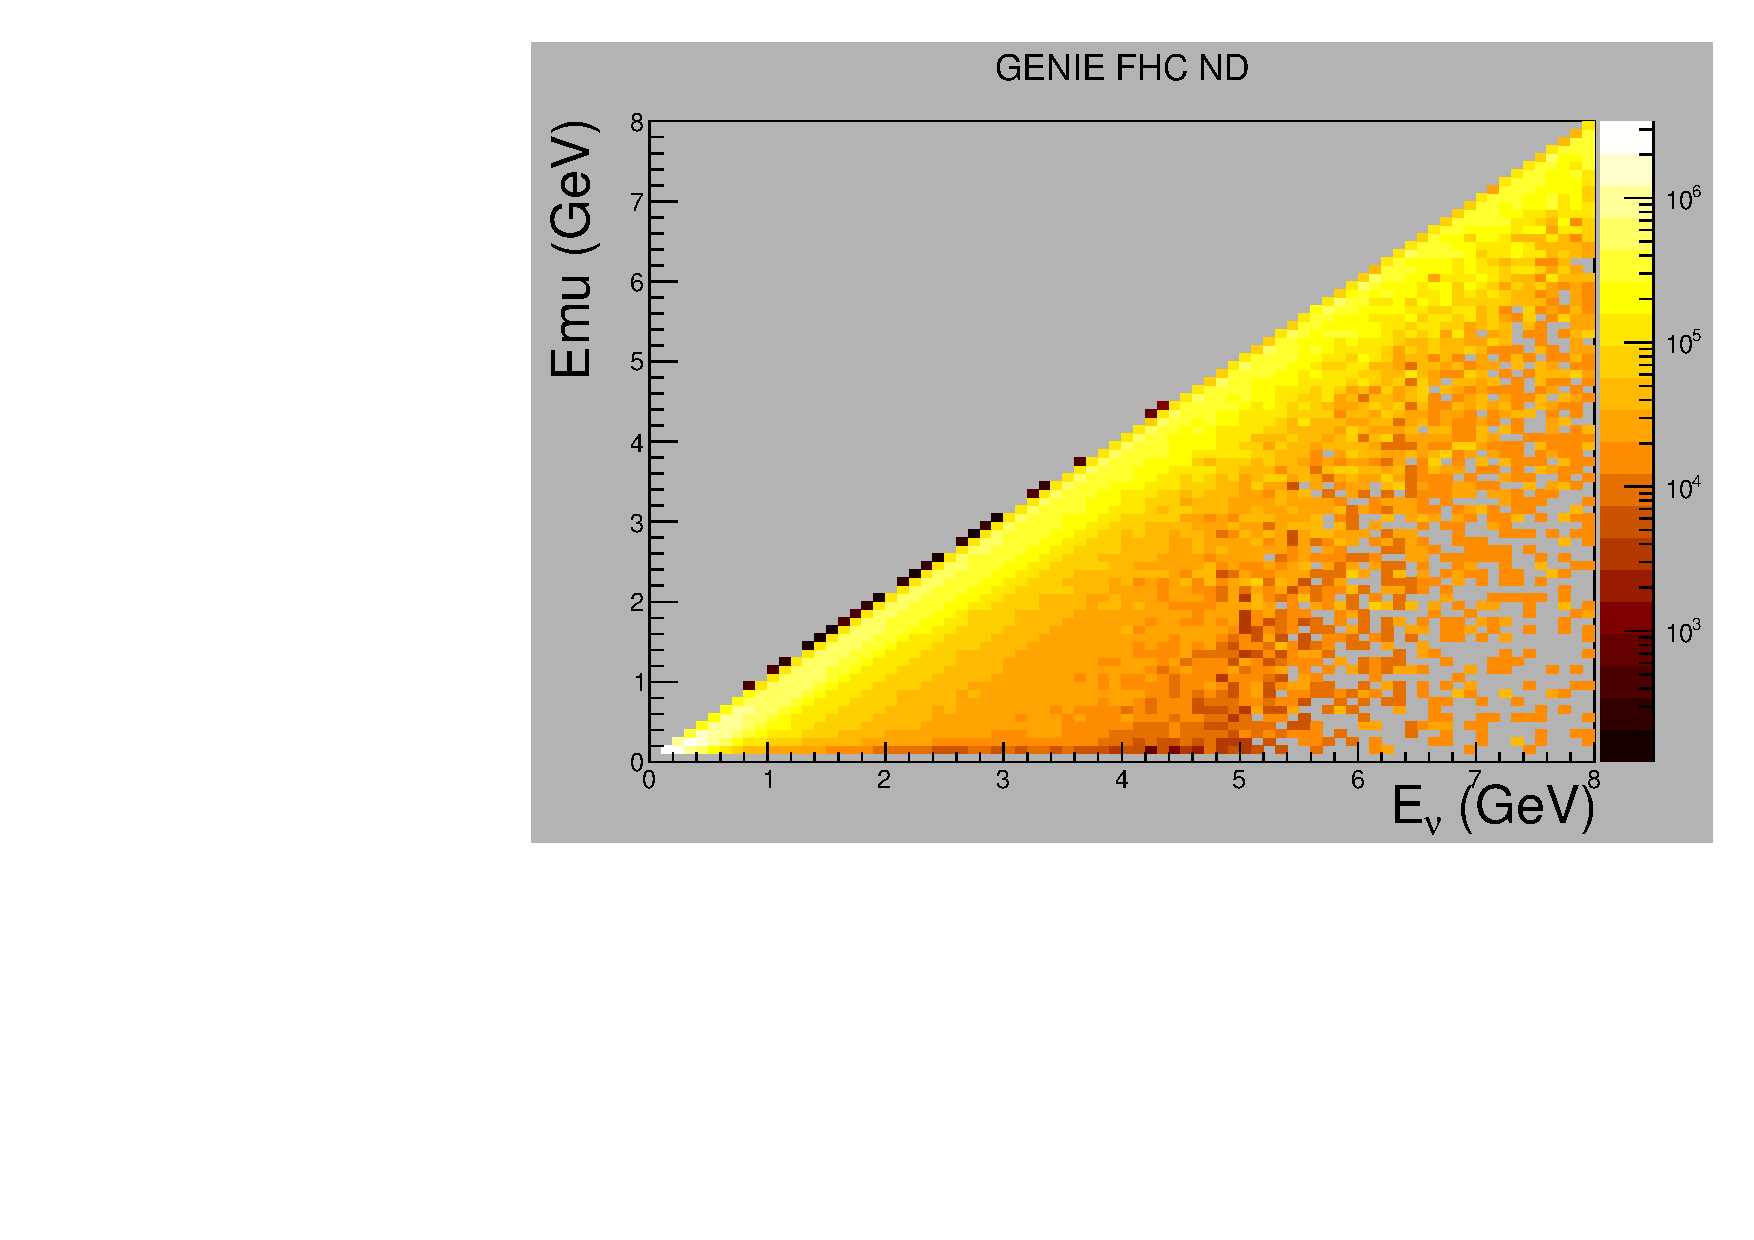
\includegraphics[width=0.5\textwidth]{plots.old/fig1.pdf}
  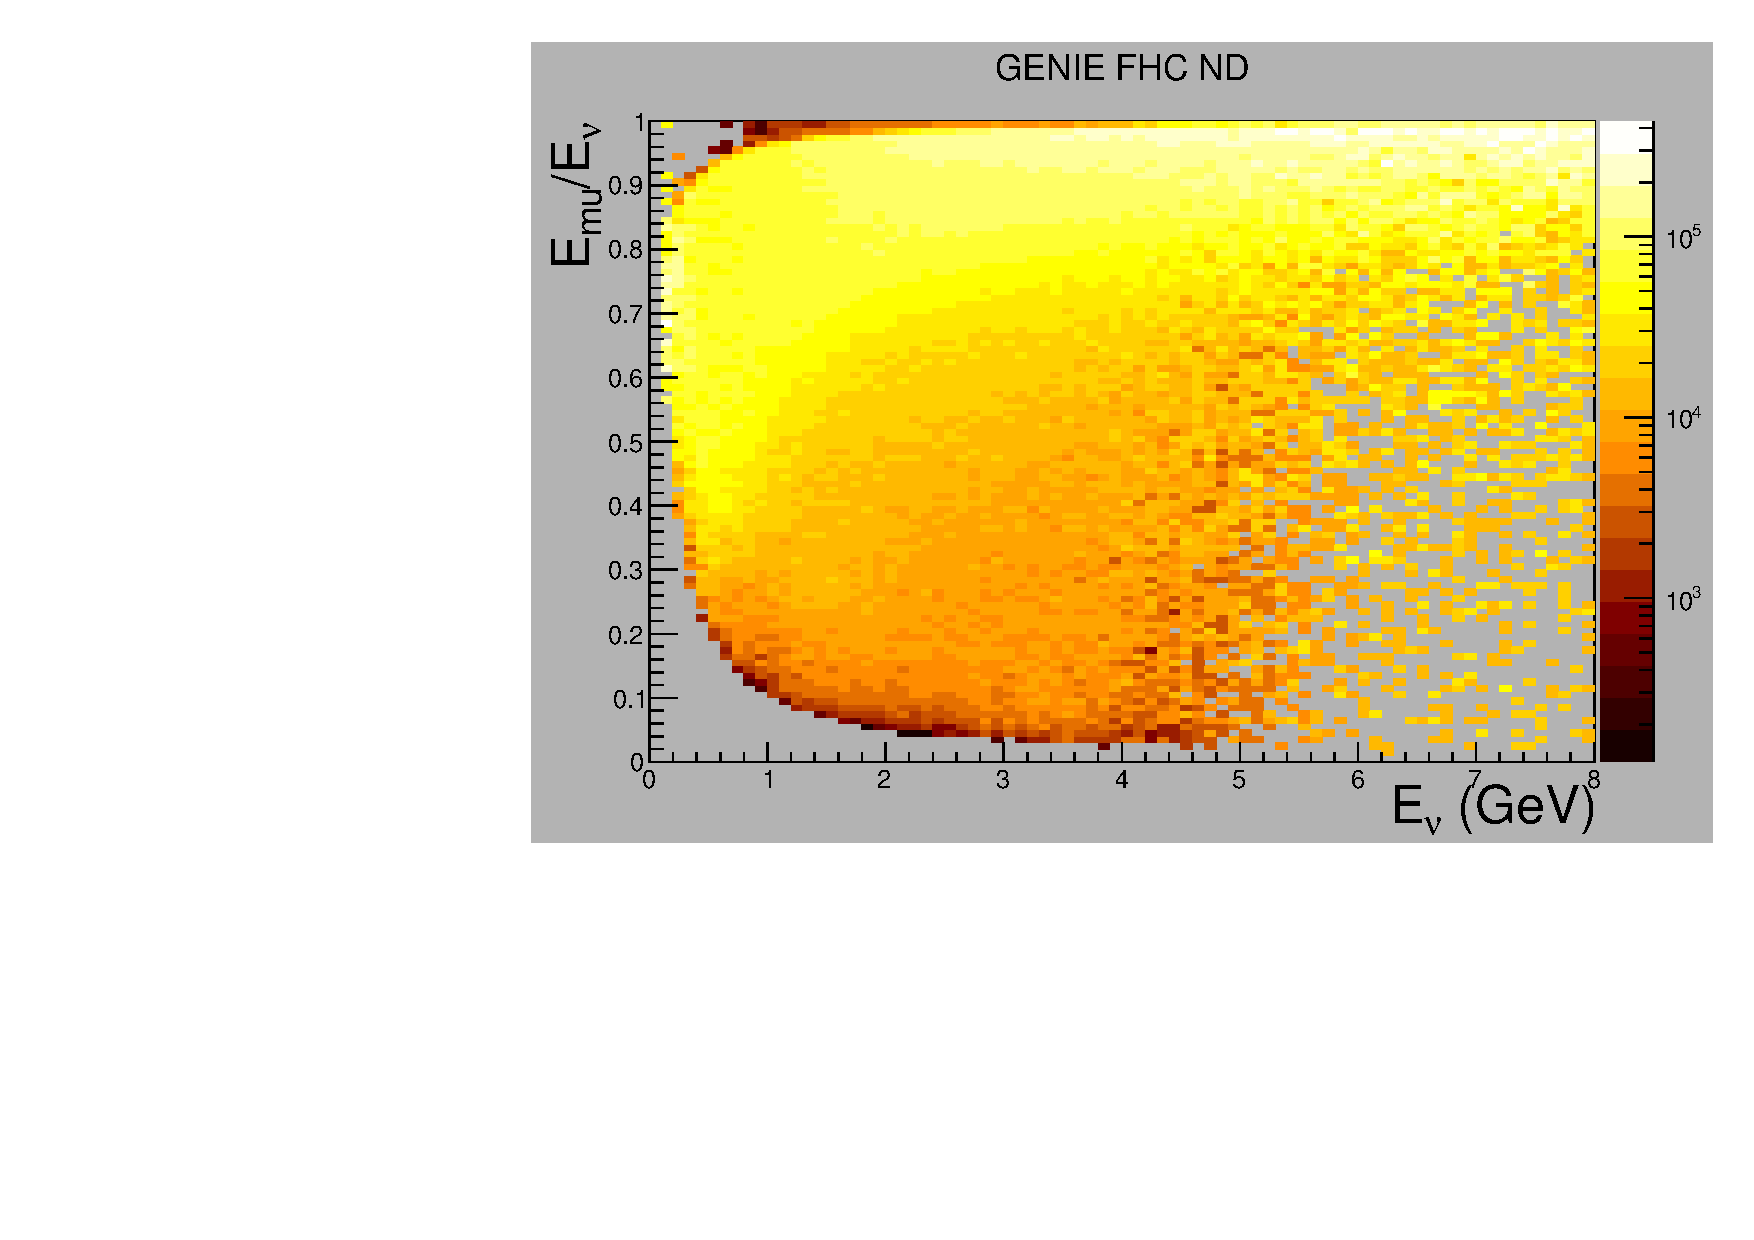
\includegraphics[width=0.5\textwidth]{plots.old/fig2.pdf}
  \caption{Flux-normalized energy distribution of final state leptons in GENIE events on argon in 1mu0pi events.}
\end{figure}

\begin{figure}[!h]
  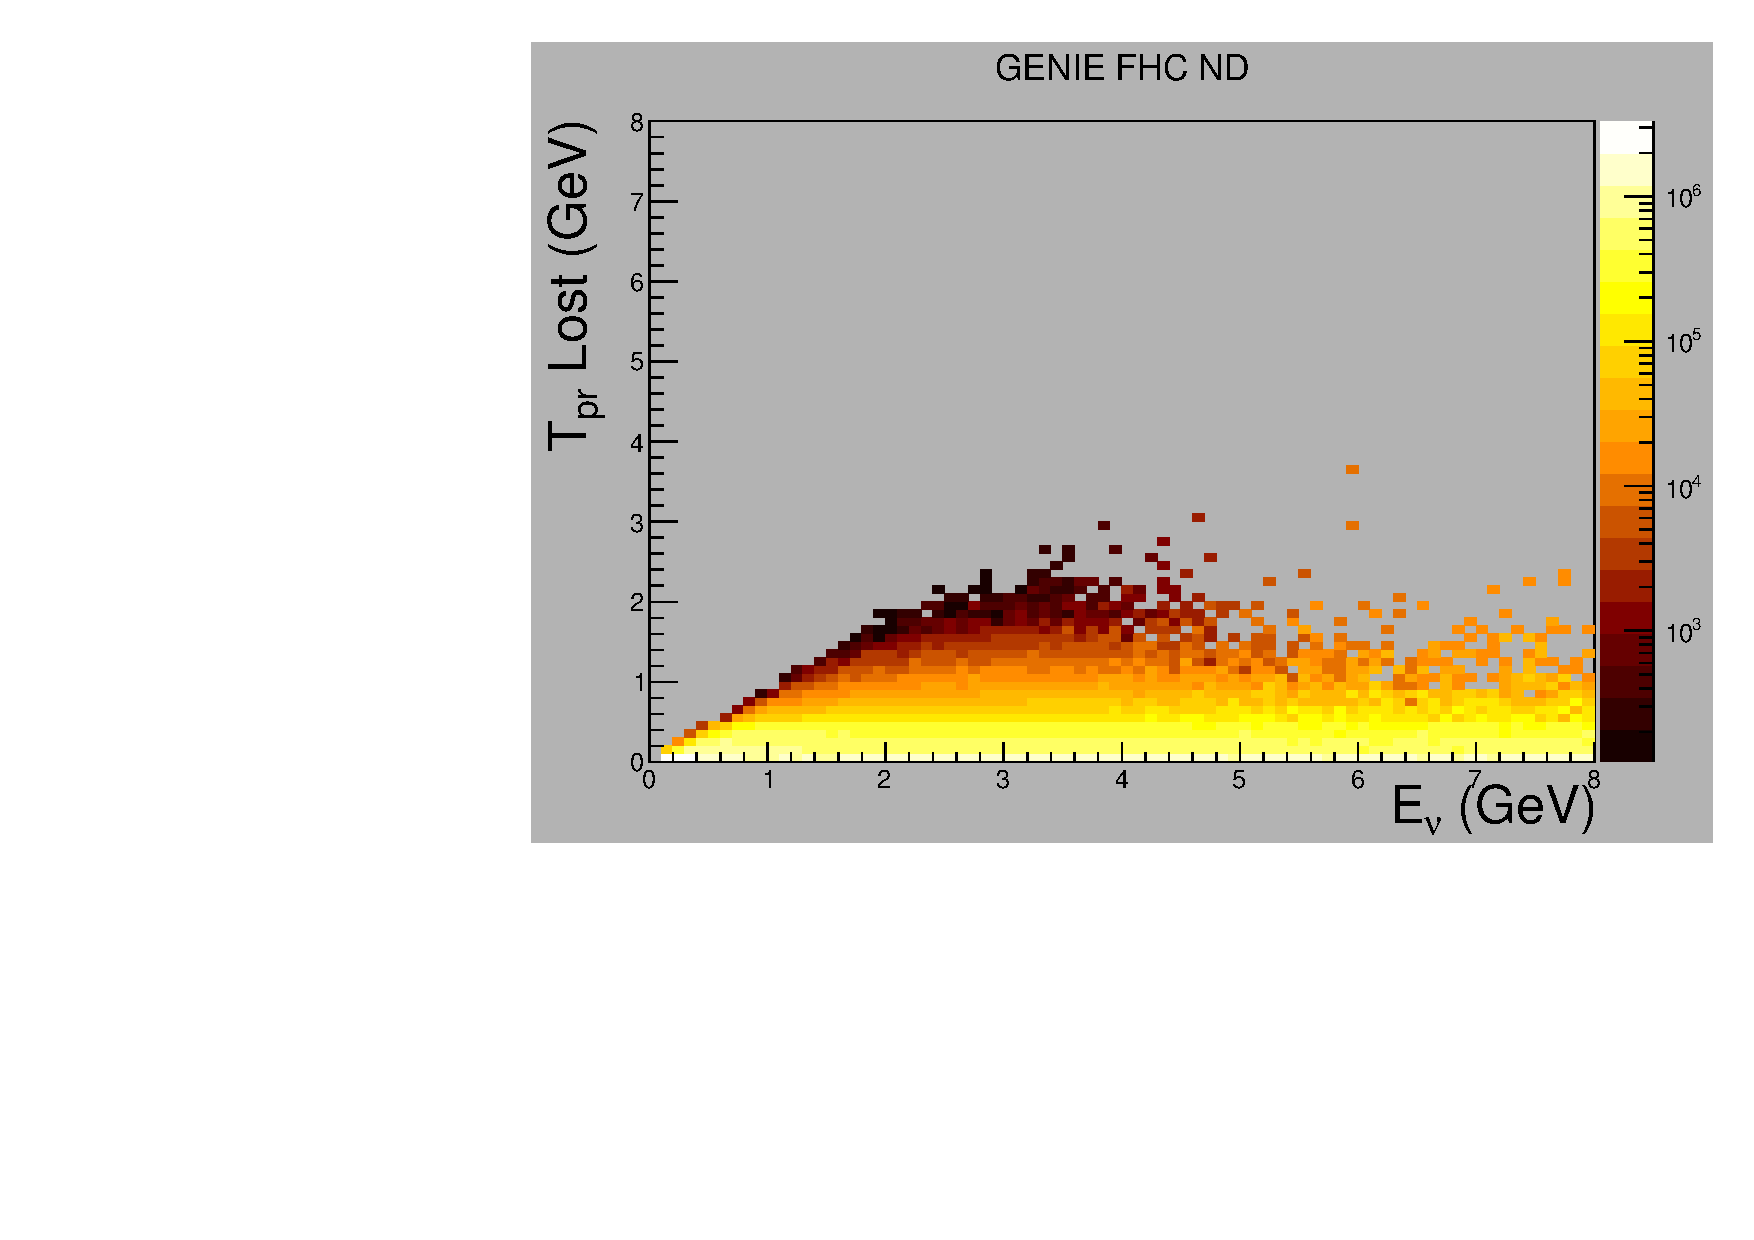
\includegraphics[width=0.5\textwidth]{plots.old/fig3.pdf}
  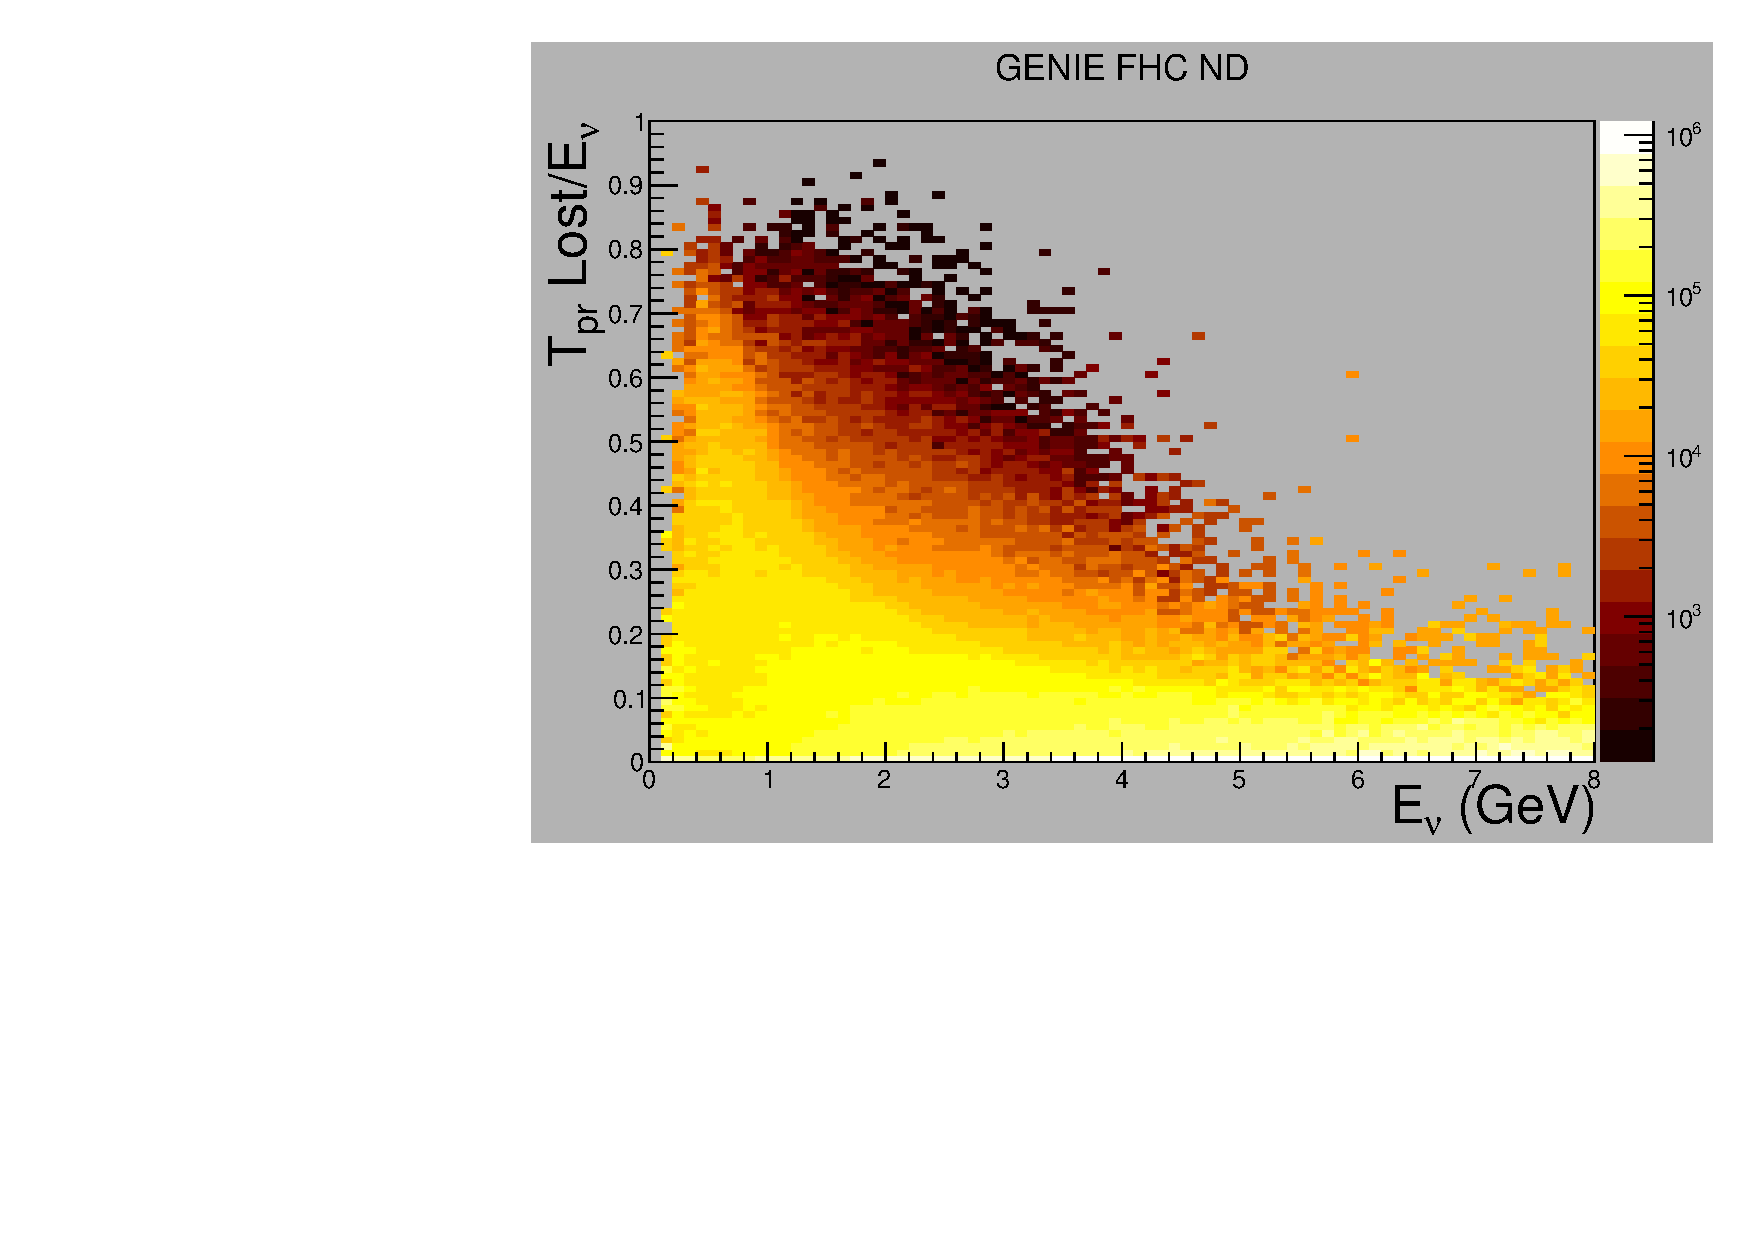
\includegraphics[width=0.5\textwidth]{plots.old/fig4.pdf}
  \caption{Flux-normalized energy distribution of final state protons in GENIE events on argon in 1mu0pi events.}
\end{figure}

\begin{figure}[!h]
  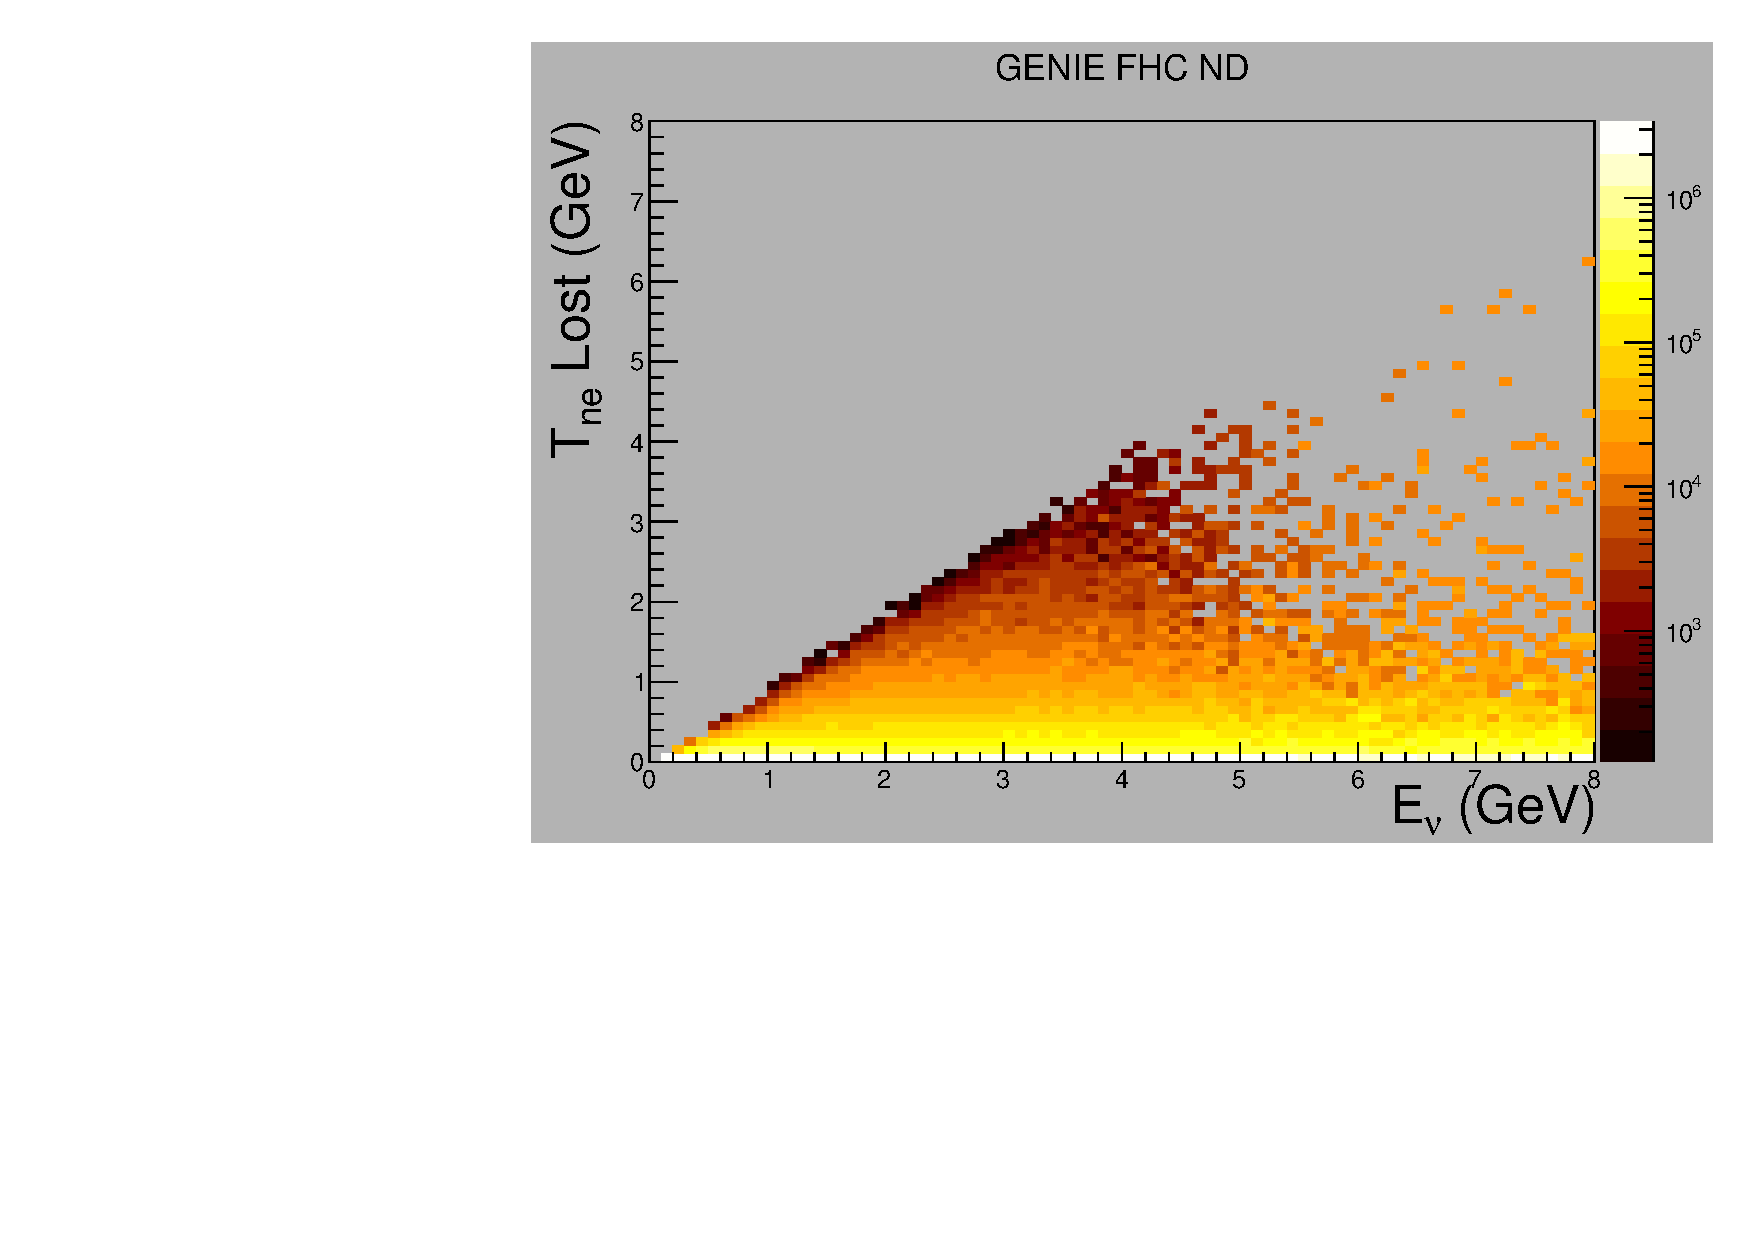
\includegraphics[width=0.5\textwidth]{plots.old/fig5.pdf}
  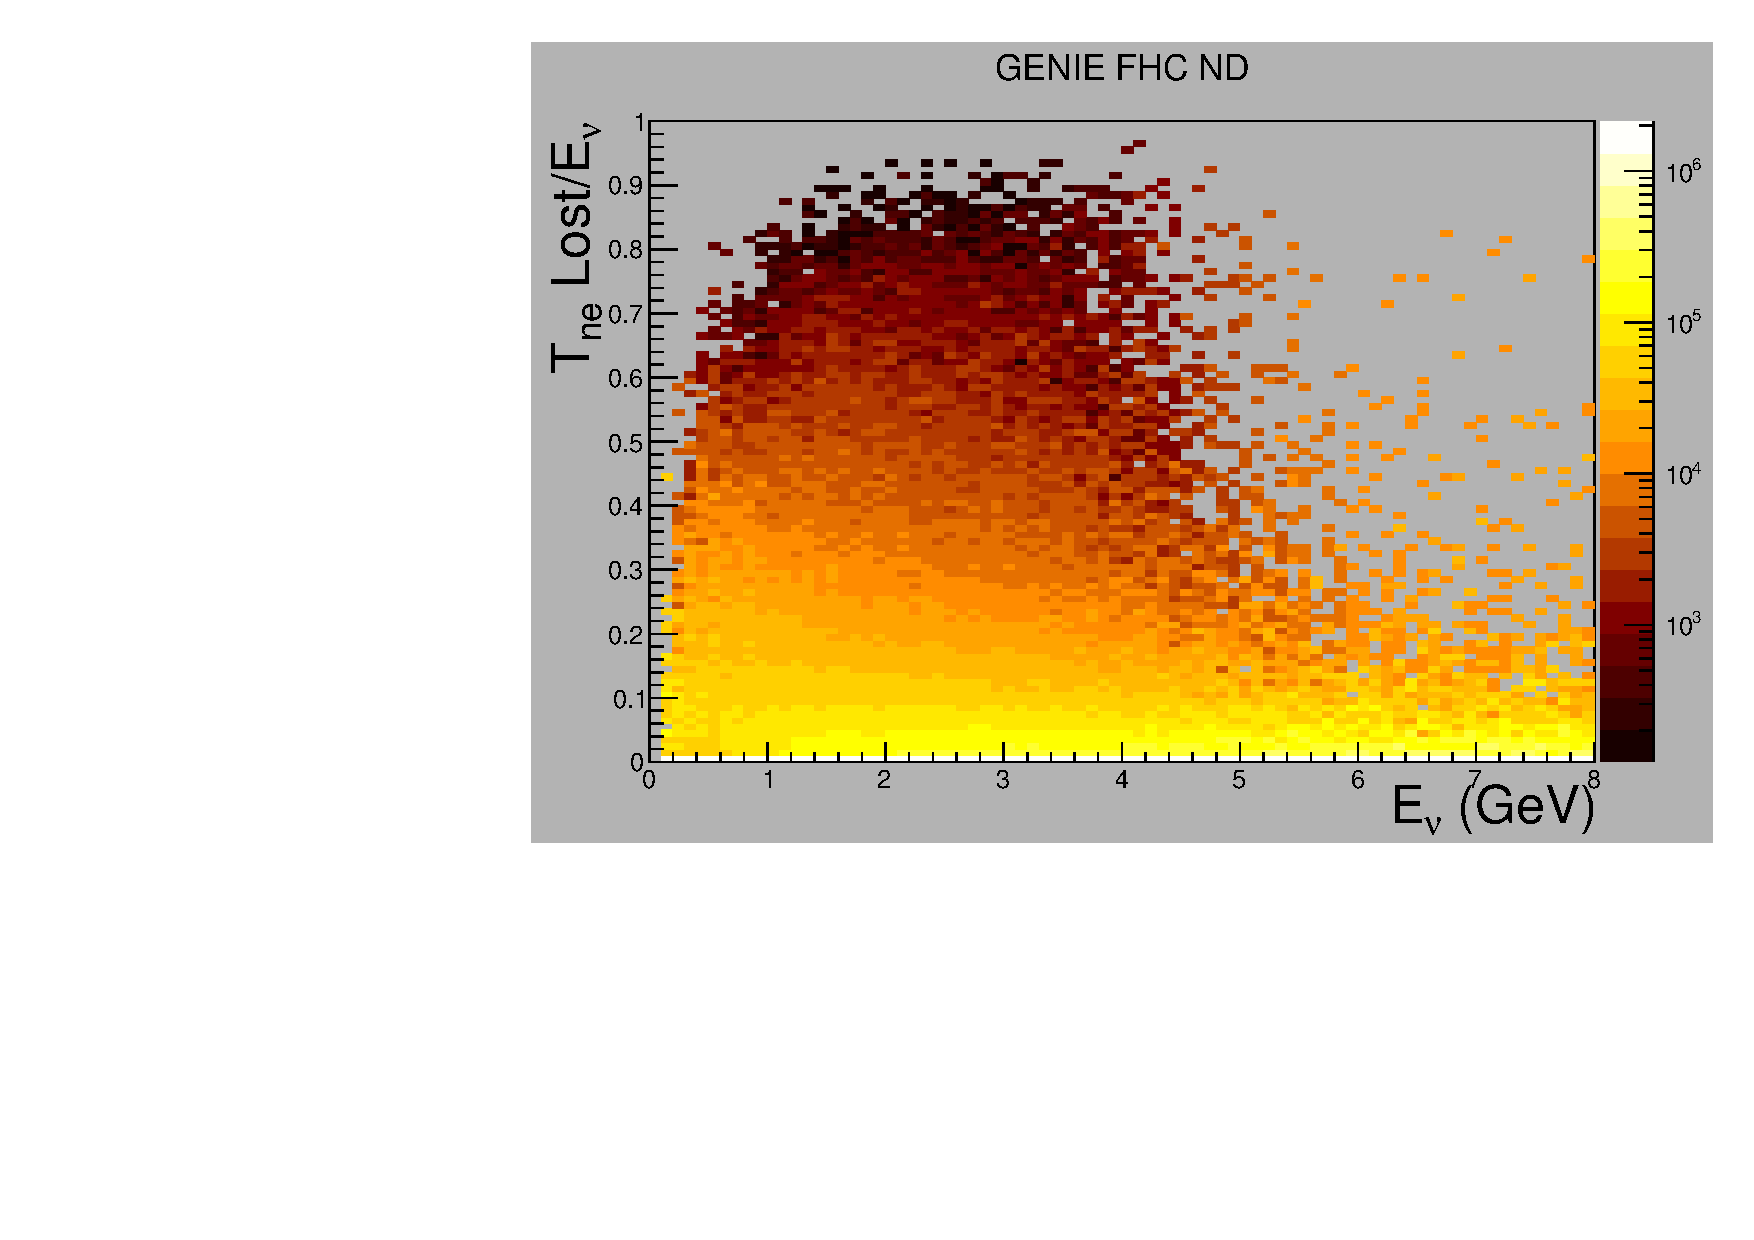
\includegraphics[width=0.5\textwidth]{plots.old/fig6.pdf}
  \caption{Flux-normalized energy distribution of final state neutrons in GENIE events on argon in 1mu0pi events.}
\end{figure}

%% \begin{figure}[!h]
%%   \includegraphics[width=0.5\textwidth]{plots/threshold_1mu0pi_500MeV/pip/Epip_Enu_GENIE_FHC_ND_numu.pdf}
%%   \includegraphics[width=0.5\textwidth]{plots/threshold_1mu0pi_500MeV/pip/Epip_Enu_frac_GENIE_FHC_ND_numu.pdf}
%%   \caption{Flux-normalized energy distribution of final state $\pi^+$ in GENIE events on argon in 1mu0pi events (probably doesn't need to be included).}
%% \end{figure}

%% \begin{figure}[!h]
%%   \includegraphics[width=0.5\textwidth]{plots/threshold_1mu0pi_500MeV/pim/Epim_Enu_GENIE_FHC_ND_numu.pdf}
%%   \includegraphics[width=0.5\textwidth]{plots/threshold_1mu0pi_500MeV/pim/Epim_Enu_frac_GENIE_FHC_ND_numu.pdf}
%%   \caption{Flux-normalized energy distribution of final state $\pi^-$ in GENIE events on argon in 1mu0pi events (probably doesn't need to be included).}
%% \end{figure}

%% \begin{figure}[!h]
%%   \includegraphics[width=0.5\textwidth]{plots/threshold_1mu0pi_500MeV/pi0/Epi0_Enu_GENIE_FHC_ND_numu.pdf}
%%   \includegraphics[width=0.5\textwidth]{plots/threshold_1mu0pi_500MeV/pi0/Epi0_Enu_frac_GENIE_FHC_ND_numu.pdf}
%%   \caption{Flux-normalized energy distribution of final state $\pi^0$ in GENIE events on argon in 1mu0pi events (probably doesn't need to be included).}
%% \end{figure}

\subsection{Hard Threshold}

The final state kinematics depend heavily upon the true final state particles, so we selected samples based on this information.  We looked at the following samples:

\begin{itemize}
\item 1 muon, 1 proton
\item 1 muon, multiple protons
\item 1 muon, 1 charged pion
\item 1 muon, no charged pions
\end{itemize}

We'll examine the 1 muon 0 charged pion case as an example before presenting the rest of the plots.

We impose a hard threshold on the kinetic energy of the proton and charged pions.  We accept all muons, all neutral pions, and assume no sensitivity for neutrons.

With this cut, we can examine the detected energy of each event:

\begin{align}
  E_{\mathrm{reco}} = E_{\mu} + T_{p \; \mathrm{passed}} + E_{\pi^{\pm} \; \mathrm{passed}} + E_{\pi^0}
\end{align}

\begin{figure}[!h]
  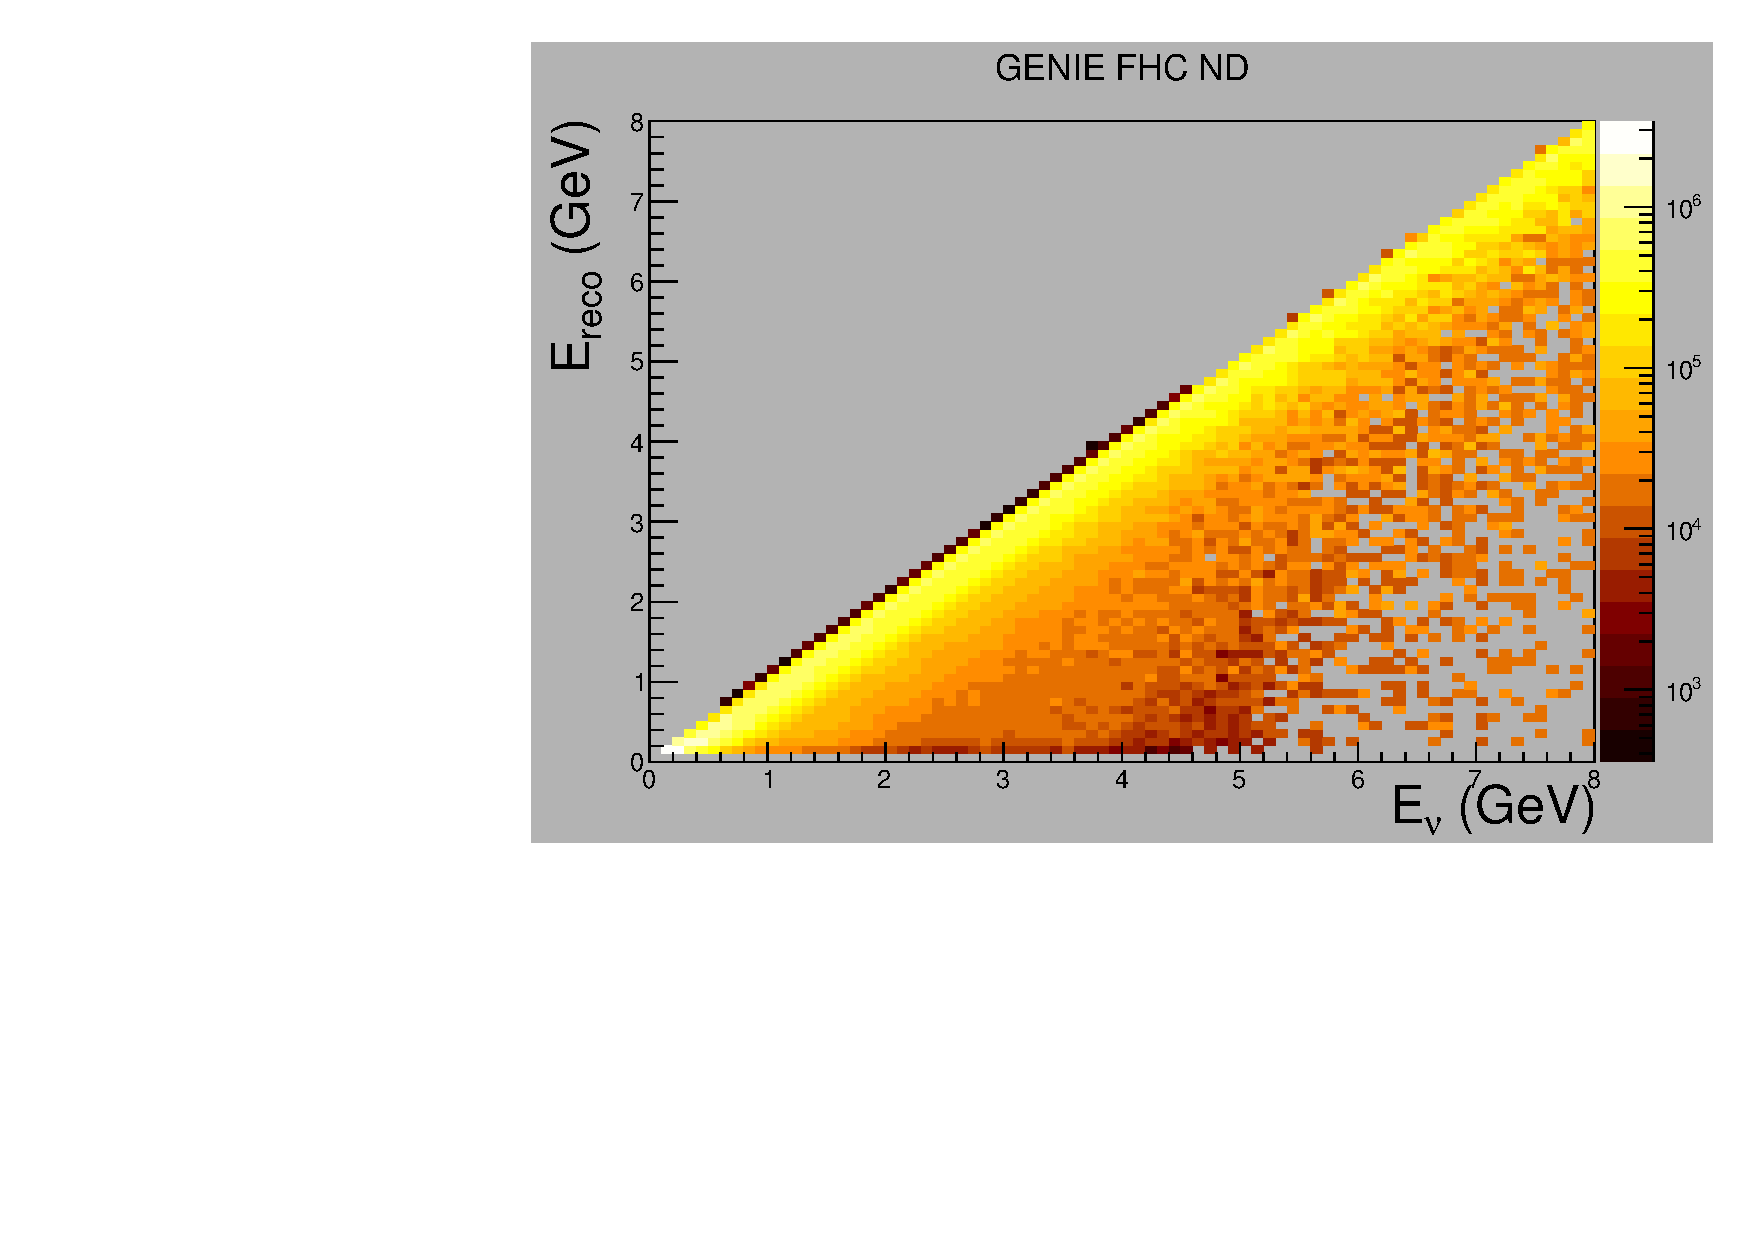
\includegraphics[width=0.5\textwidth]{plots.old/fig7.pdf}
  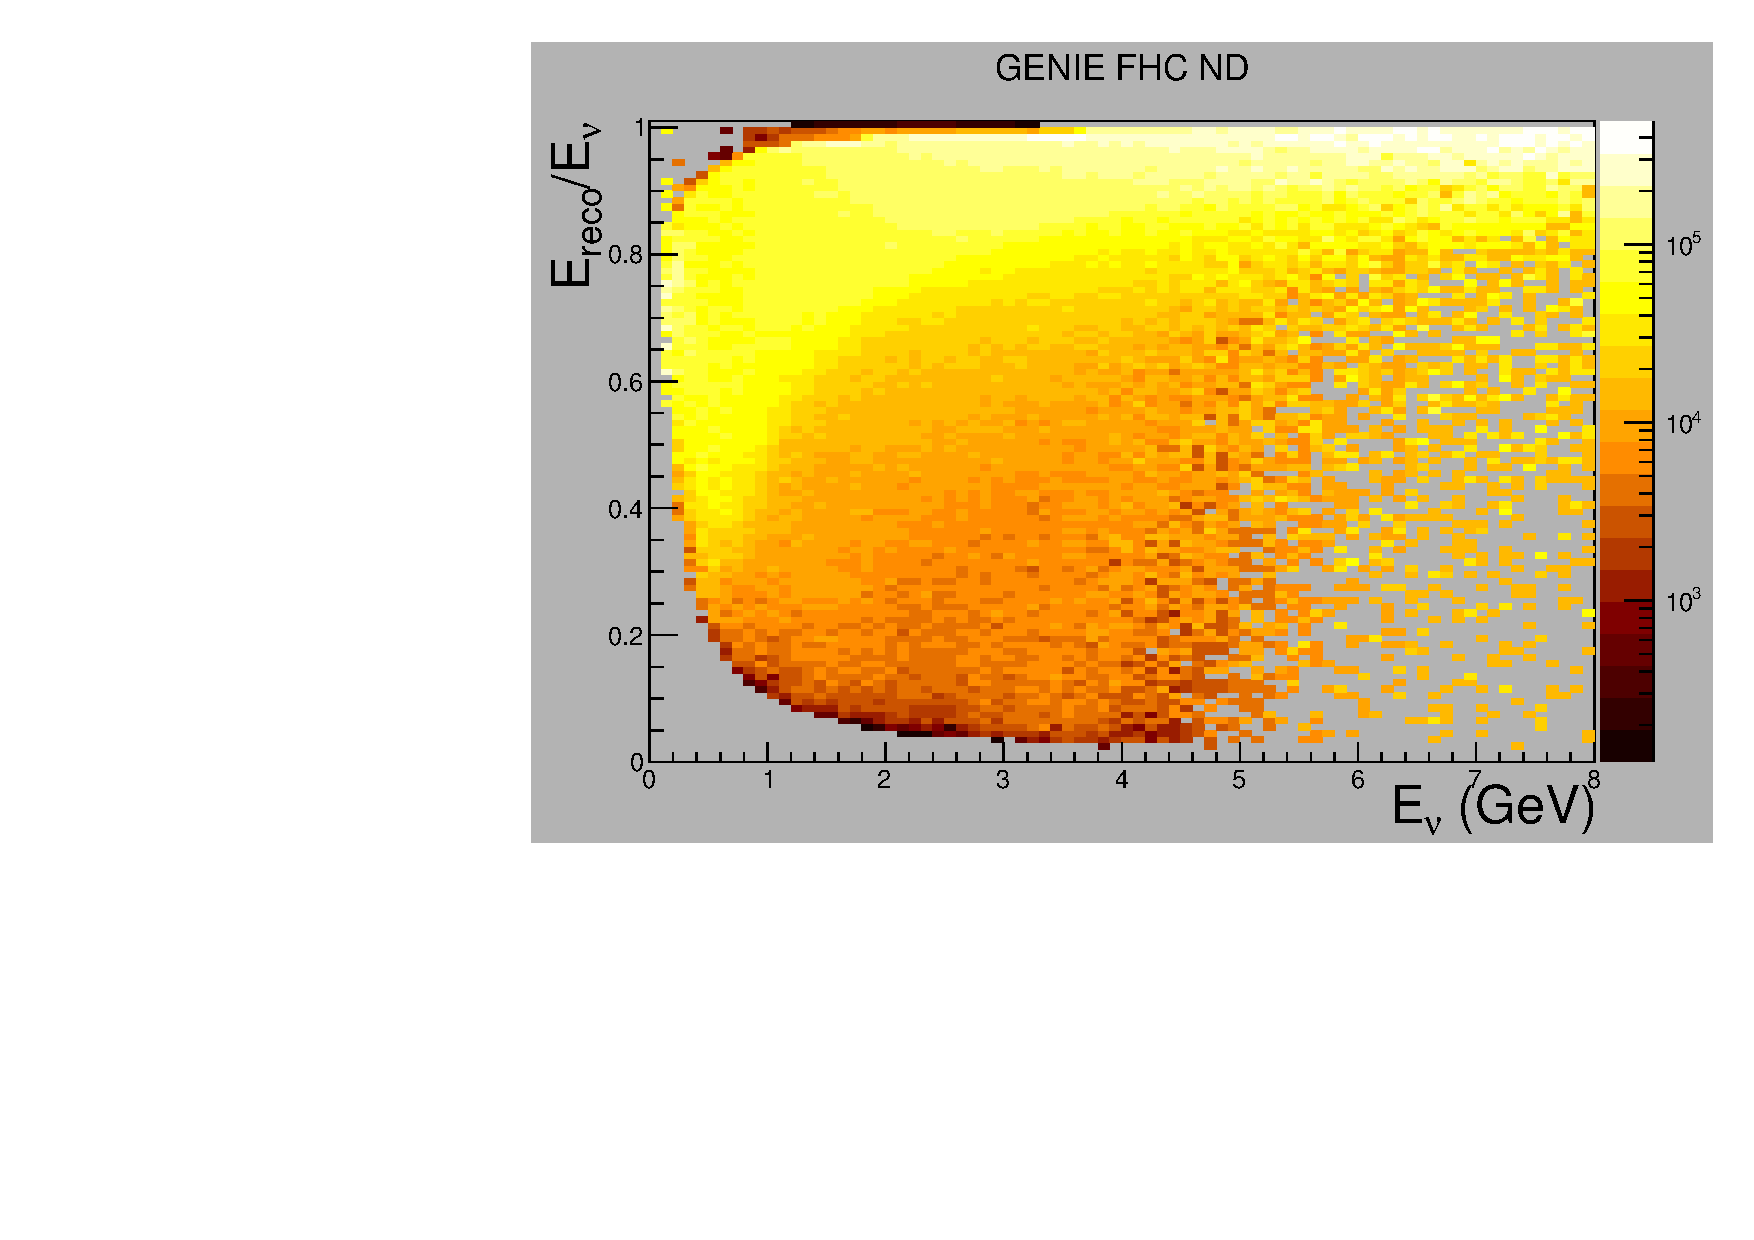
\includegraphics[width=0.5\textwidth]{plots.old/fig8.pdf}
  \caption{$E_{\mathrm{reco}}$ vs. $E_\nu$ shown for GENIE events on argon with a threshold of 500 MeV.}
\end{figure}

\begin{figure}[!h]
  \begin{center}
    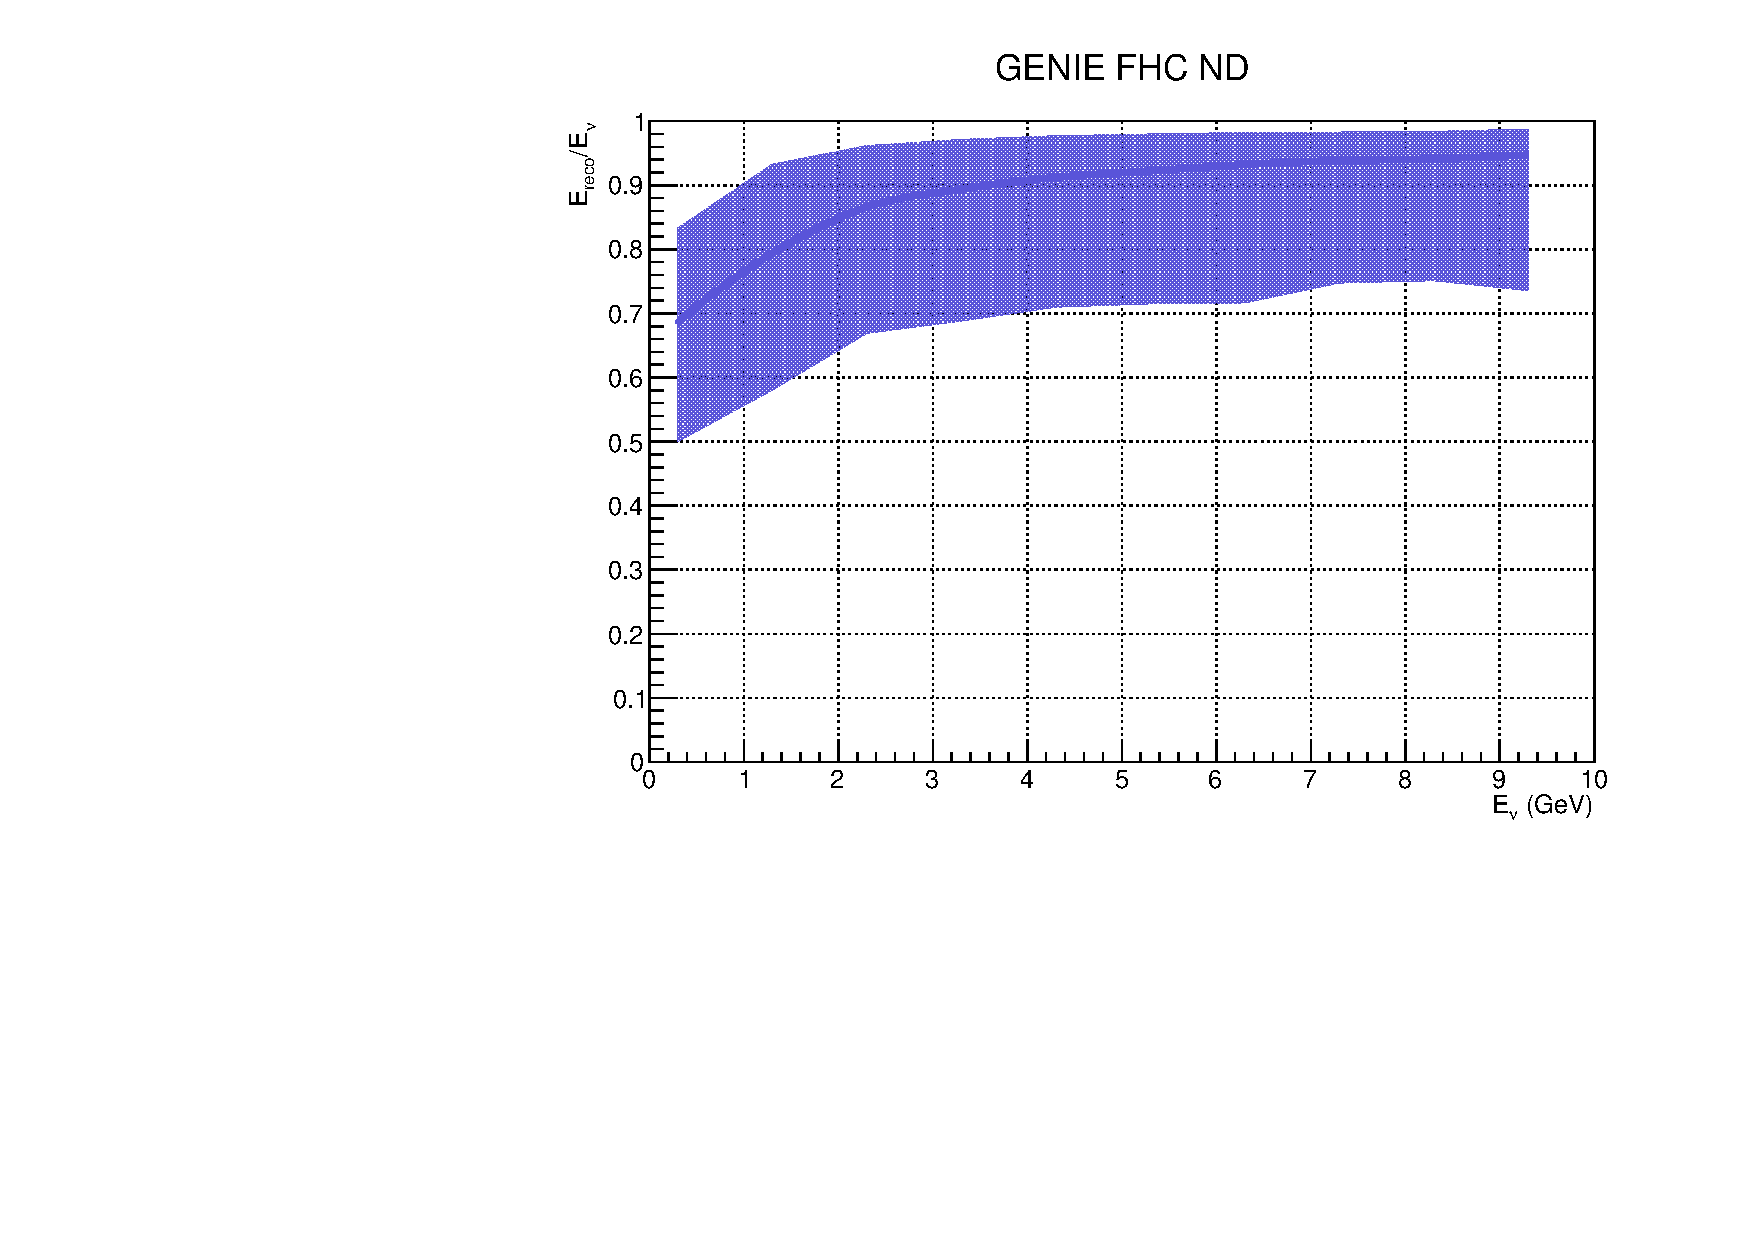
\includegraphics[width=0.7\textwidth]{plots.old/fig9.pdf}
    \caption{Median $E_{\mathrm{reco}}/E_\nu$ vs. $E_\nu$ for the above events with $68\%$ containment bands.}
  \end{center}
\end{figure}

Similarly, we can also look at the energy ``lost'' in each event:

\begin{align}
  E_{\mathrm{lost}} = T_{p \; \mathrm{failed}} + T_{n} + E_{\pi^{\pm} \; \mathrm{lost}}
\end{align}

Which (assuming no $\gamma$s are produced), should be such that $E_\nu = E_{\mathrm{lost}} + E_{\mathrm{reco}}$.

\begin{figure}[!h]
  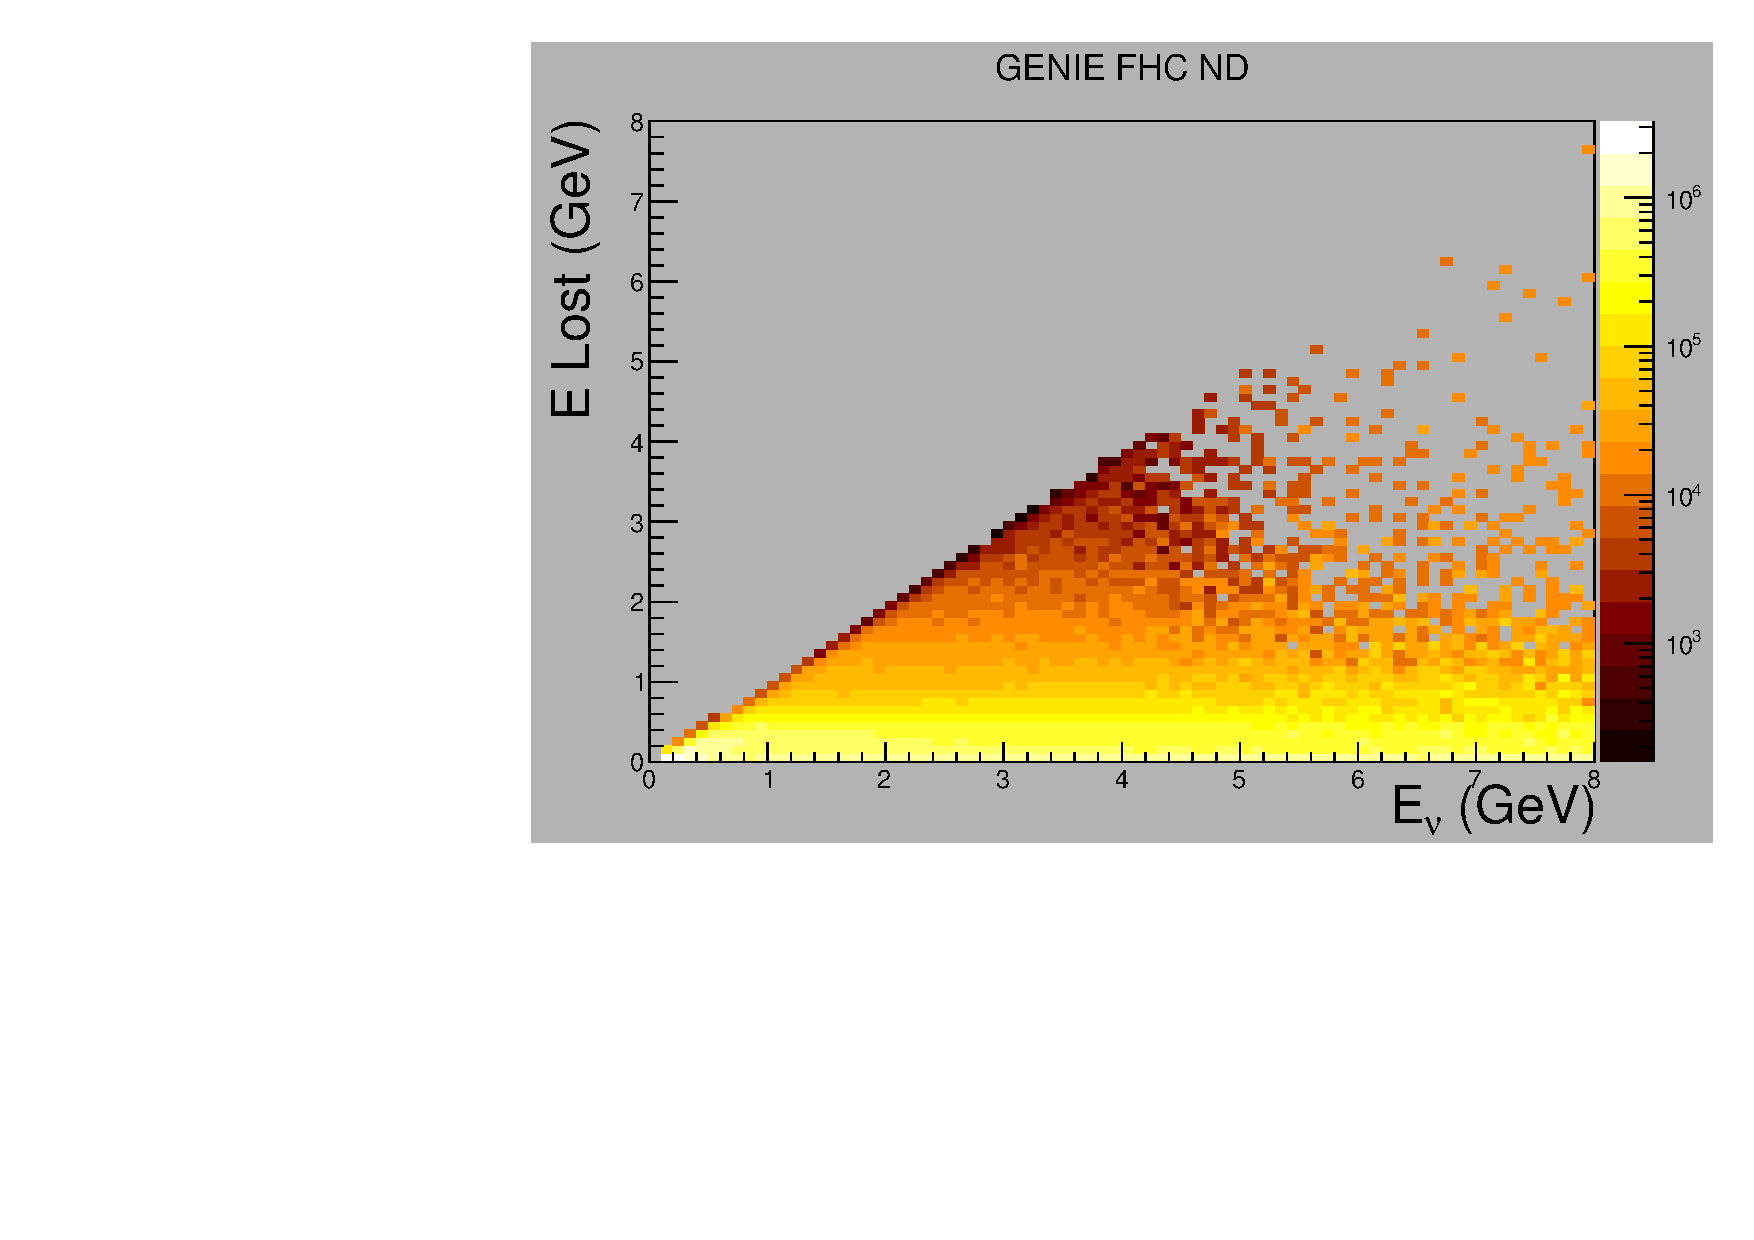
\includegraphics[width=0.5\textwidth]{plots.old/fig10.pdf}
  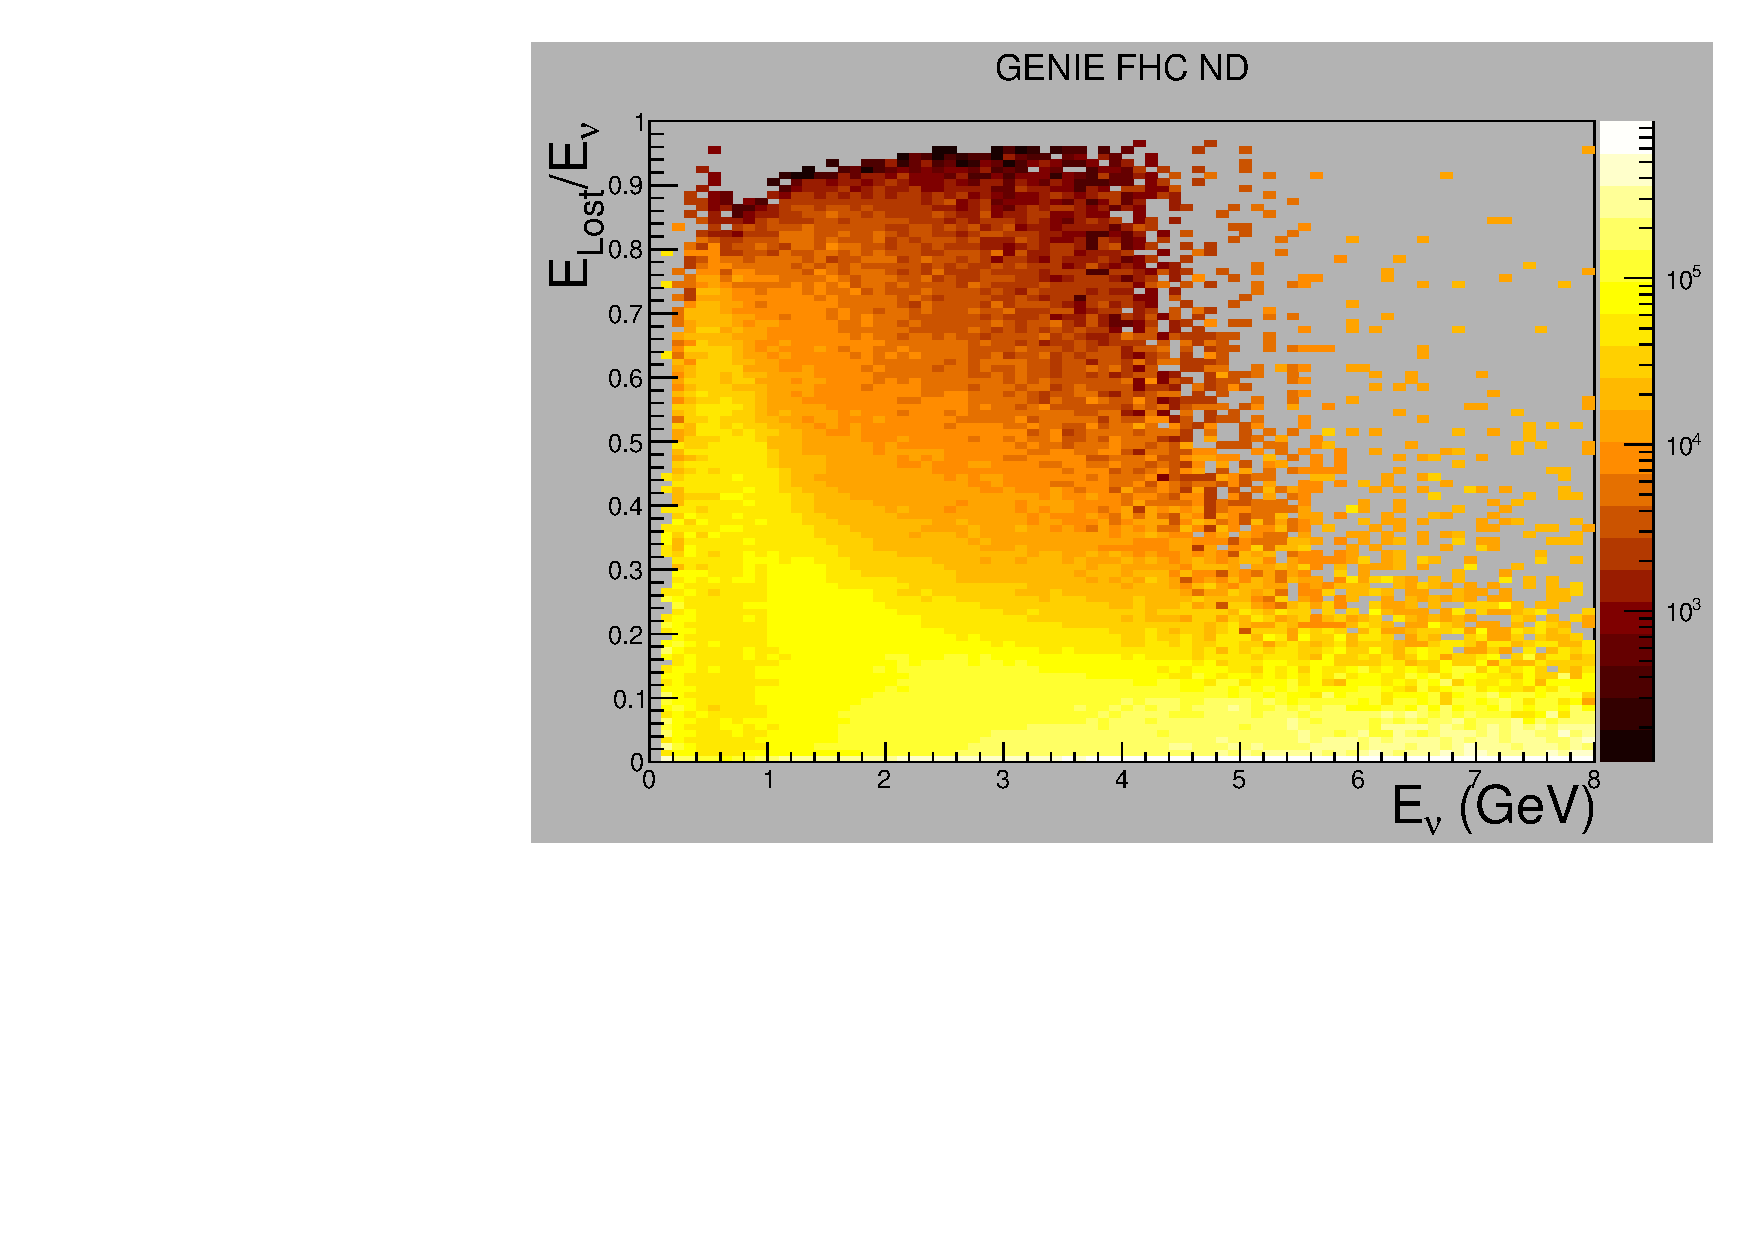
\includegraphics[width=0.5\textwidth]{plots.old/fig11.pdf}
  \caption{$E_{\mathrm{lost}}$ vs. $E_\nu$ shown for GENIE events on argon with a threshold of 500 MeV.}
\end{figure}

\begin{figure}[!h]
  \begin{center}
    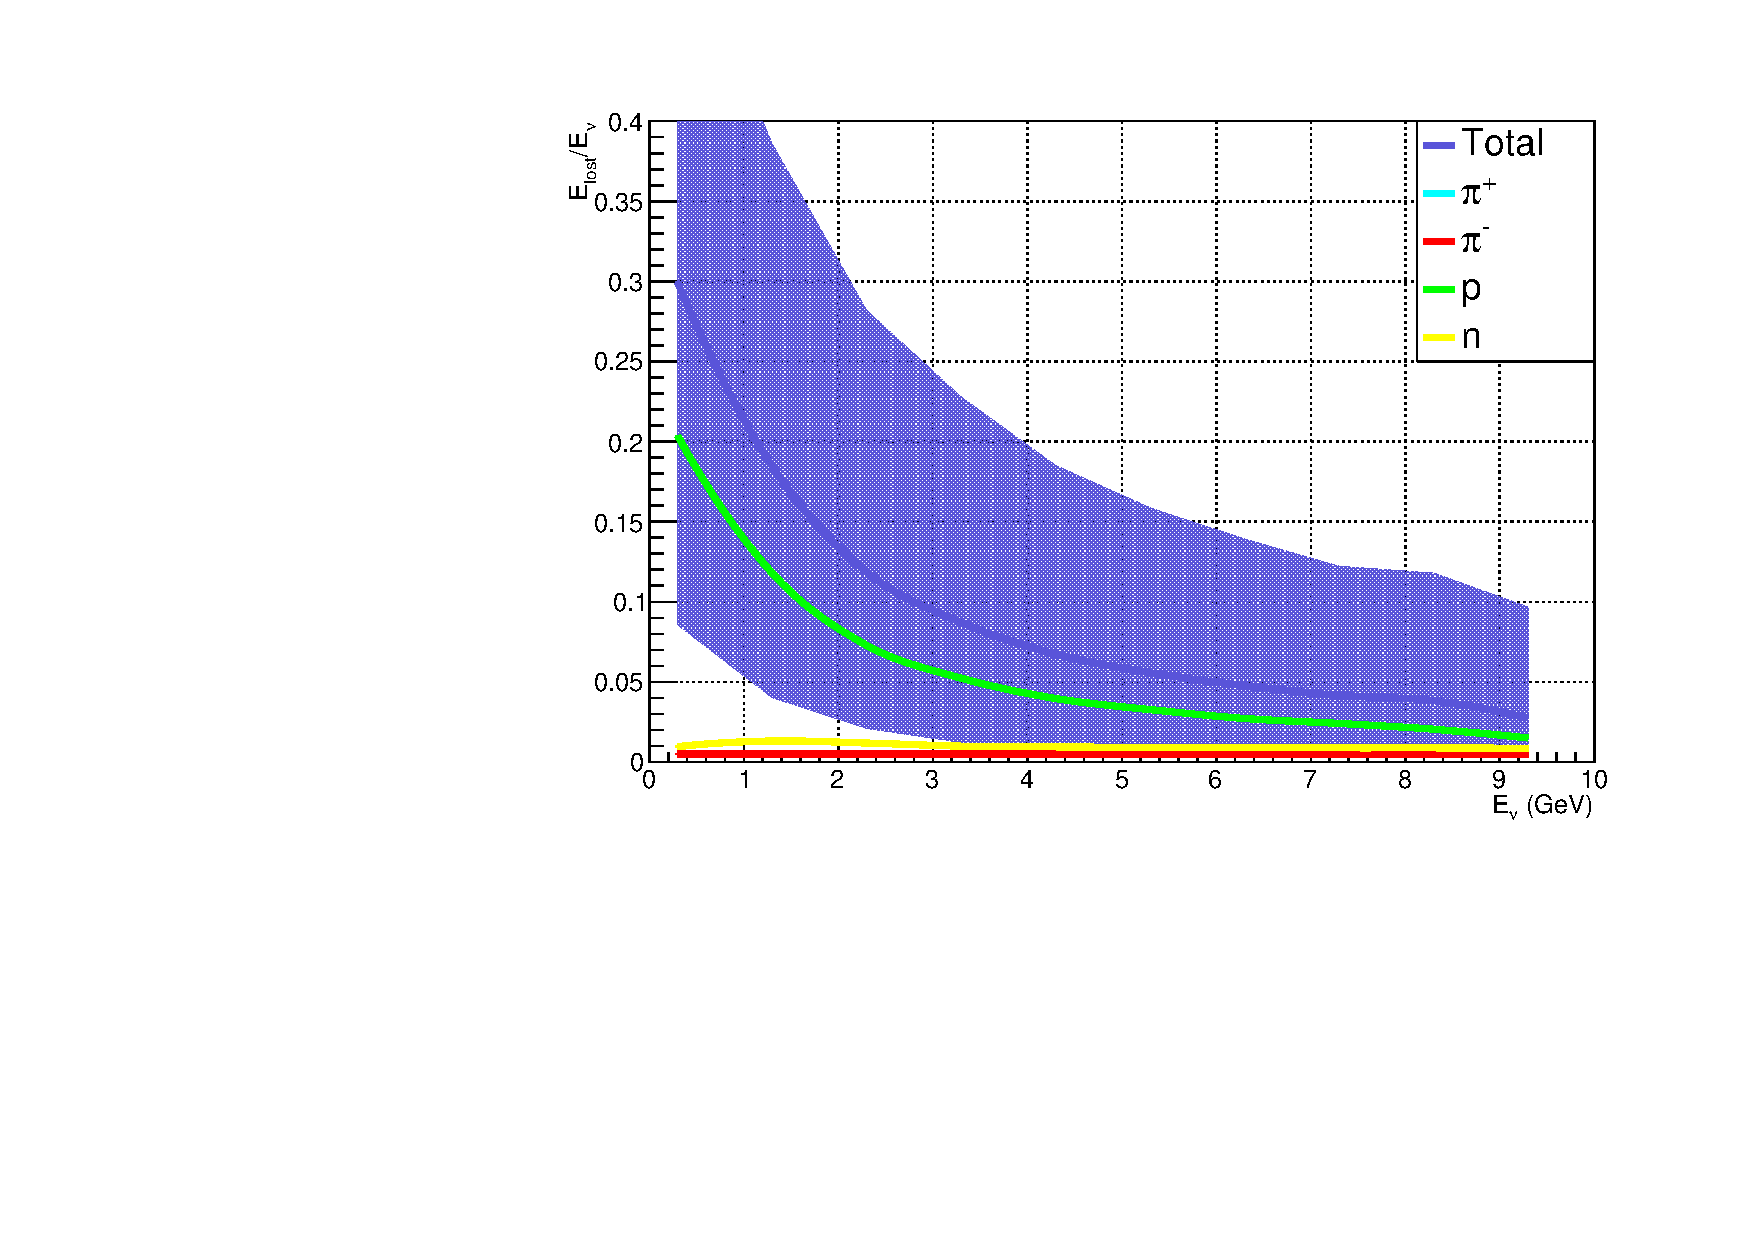
\includegraphics[width=0.7\textwidth]{plots.old/fig12.pdf}
    \caption{Median $E_{\mathrm{lost}}/E_\nu$ vs. $E_\nu$ for the above events with $68\%$ containment bands.}
  \end{center}
\end{figure}

Now it is interesting to look at the way that $E_{\mathrm{lost}}/E_\nu$ changes with a changing threshold is interesting (Figure 8).

\begin{figure}[!h]
  \begin{center}
    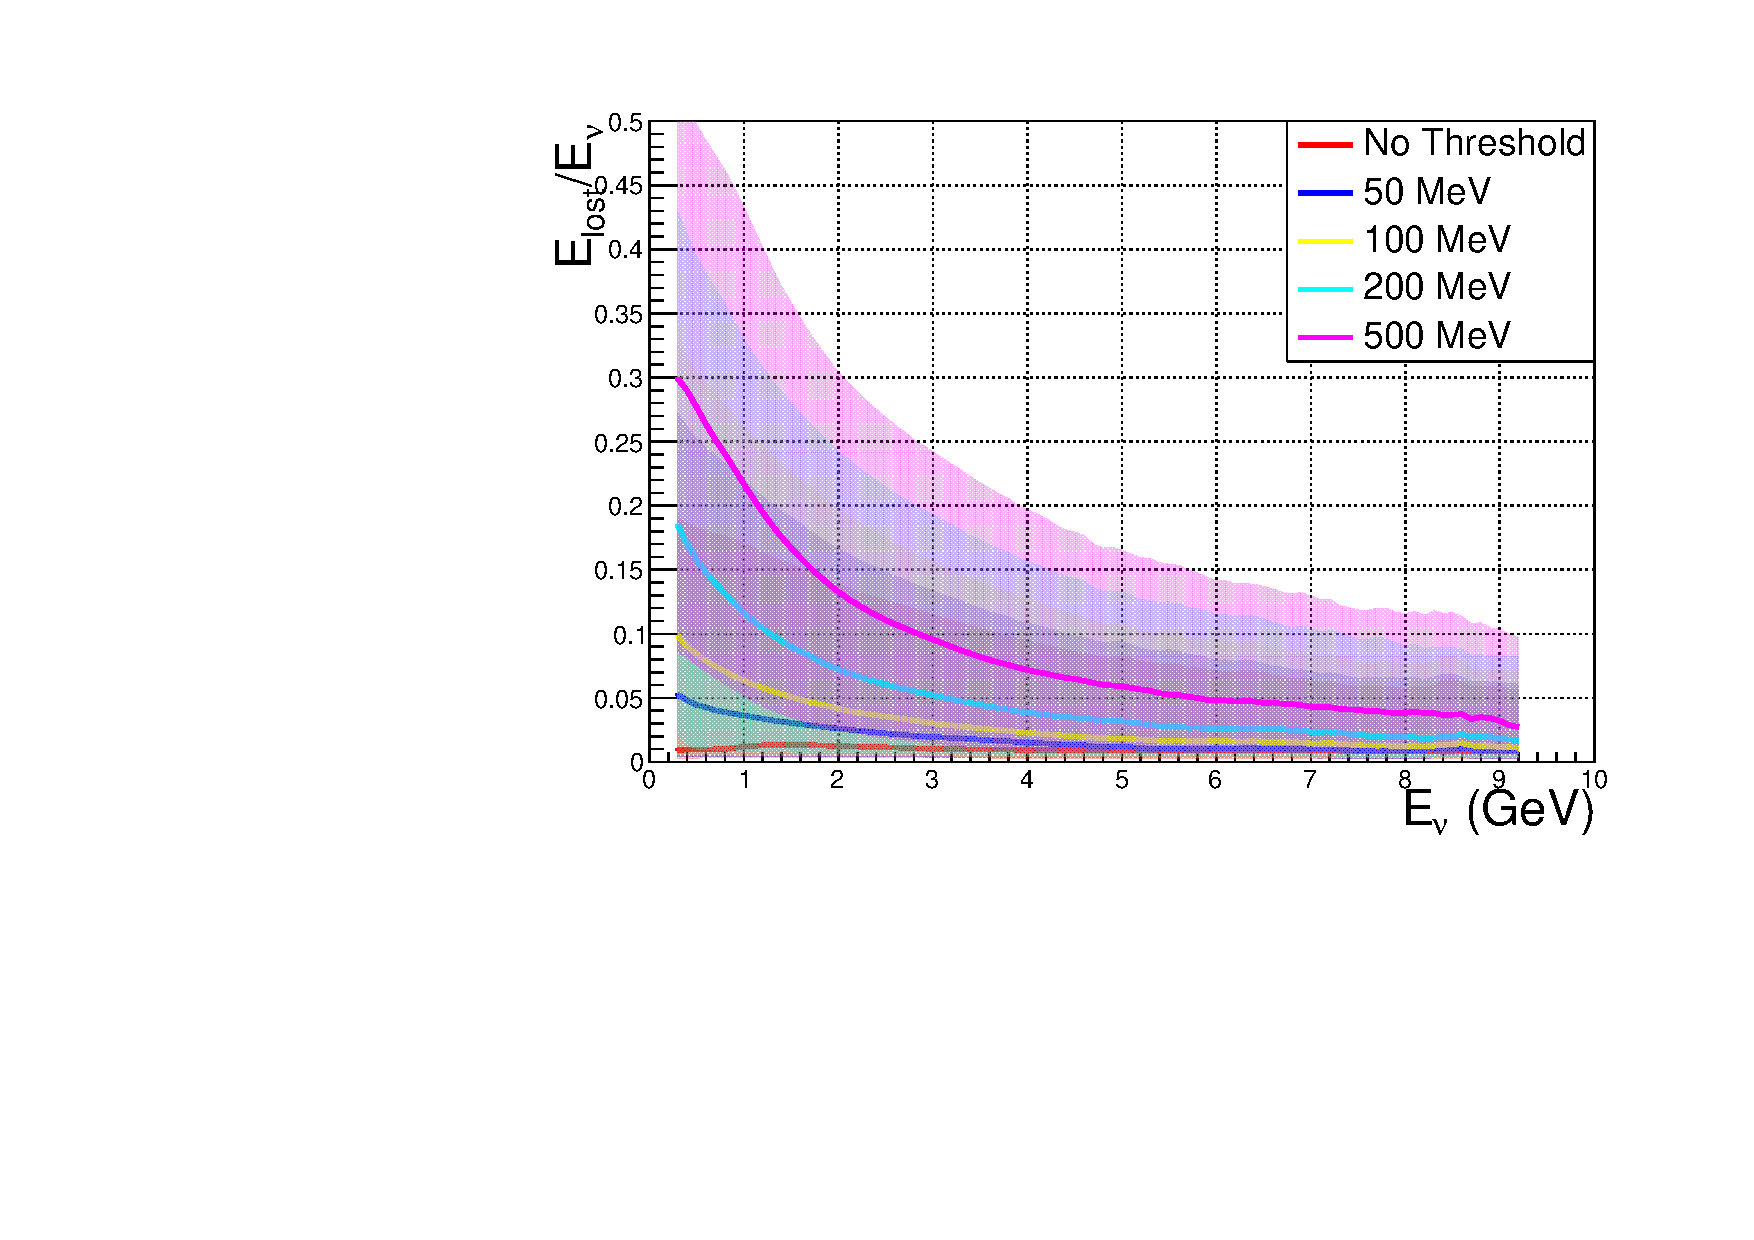
\includegraphics[width=0.7\textwidth]{plots.old/fig13.pdf}
    \caption{$E_{\mathrm{lost}}/E_\nu$ with $68\%$ containment bands for GENIE events with various thresholds.}
  \end{center}
\end{figure}

Perhaps more interesting is to examine the differences introduced when comparing the different event generators, which each use slightly different models for neutrino interaction (Figure 9).

\begin{figure}[!h]
  \begin{center}
    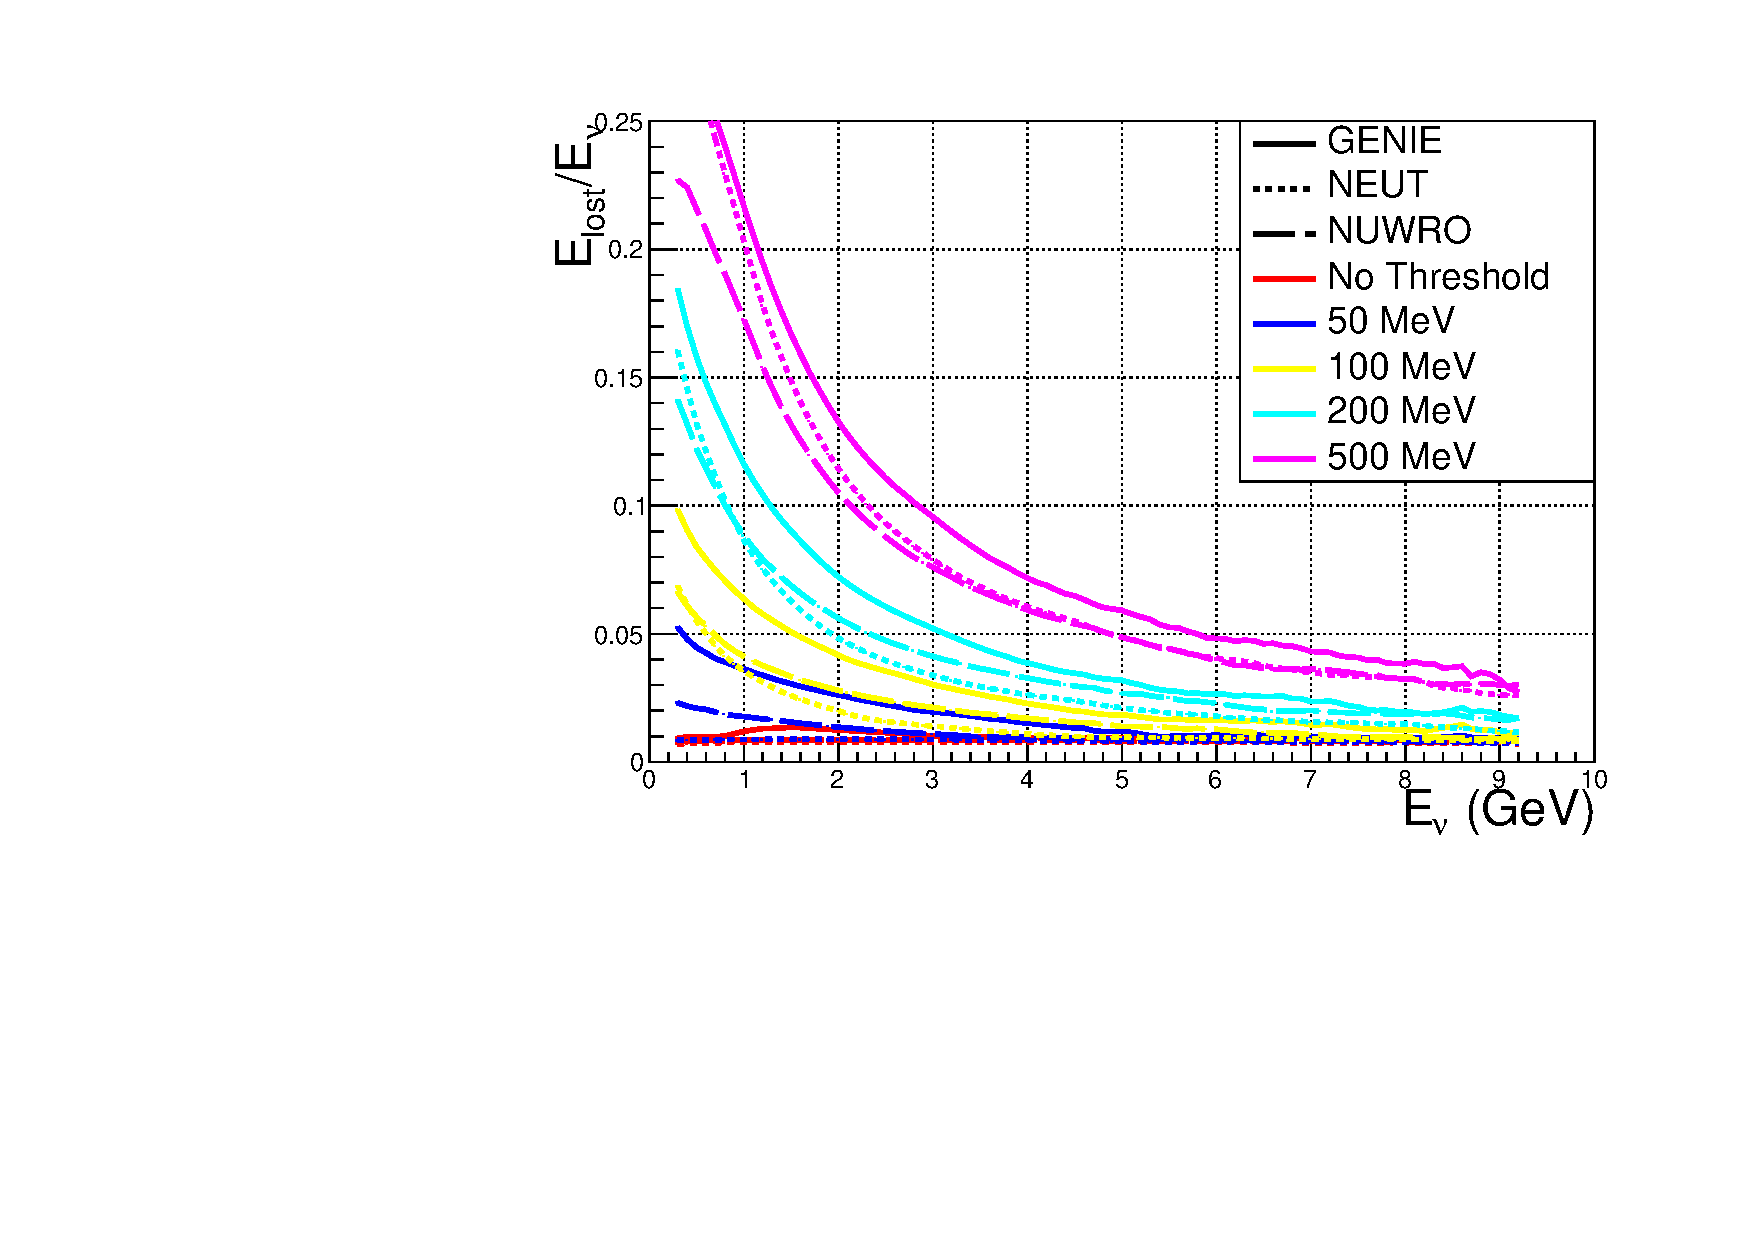
\includegraphics[width=0.7\textwidth]{plots.old/fig14.pdf}
    \caption{$E_{\mathrm{lost}}/E_\nu$ for each generator with various thresholds.}
  \end{center}
\end{figure}

\subsection{More Realistic Efficiencies}

In order to get a more realistic estimation of detector response, we need to simulate the entire detector.  Luckily, a near detector task force (NDTF) studied this problem\textsuperscript{[citation needed]} and such simulations already exist.  Unfortunately, they are only useful for the FGT detector.

%https://docs.dunescience.org/cgi-bin/private/ShowDocument?docid=1792
%NDTF report doc

\subsubsection{FGT Efficiency}

The NDTF set a fairly conservative requirement that a particle in the FGT is reconstructible if it passes through at least 12 of the straw-tubes.  Using this requirement, we are able to construct the reconstruction efficiency of the FGT using their simulation and the definition:

\begin{align}
  \eta = \frac{n_{\mathrm{passed}}}{n_{\mathrm{passed}} + n_{\mathrm{failed}}}
\end{align}

Of course, this can be binned in any way and in any (or many) kinematic variables:

\begin{figure}
  \begin{center}
    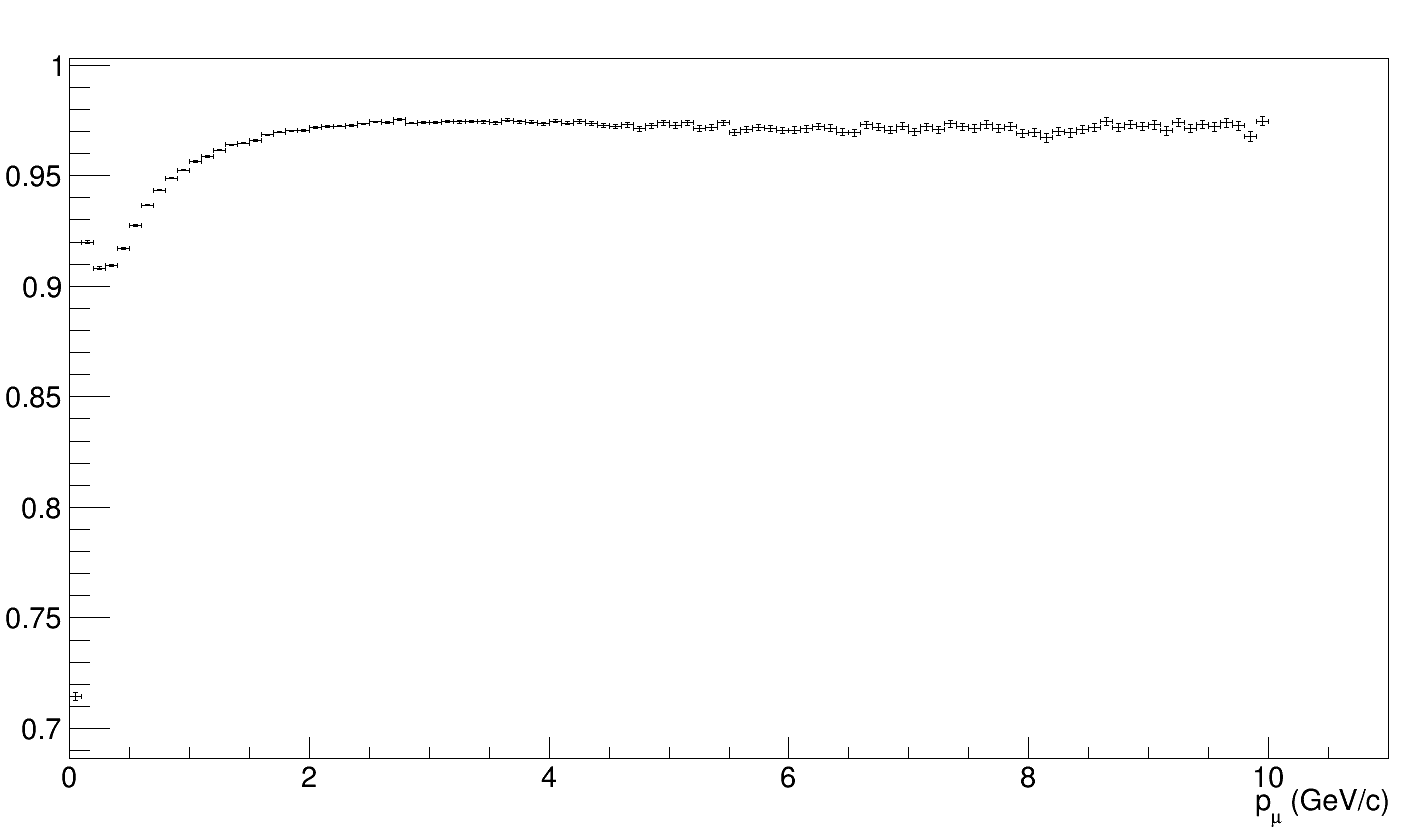
\includegraphics[width=0.45\textwidth]{plots.old/fig15.png}
    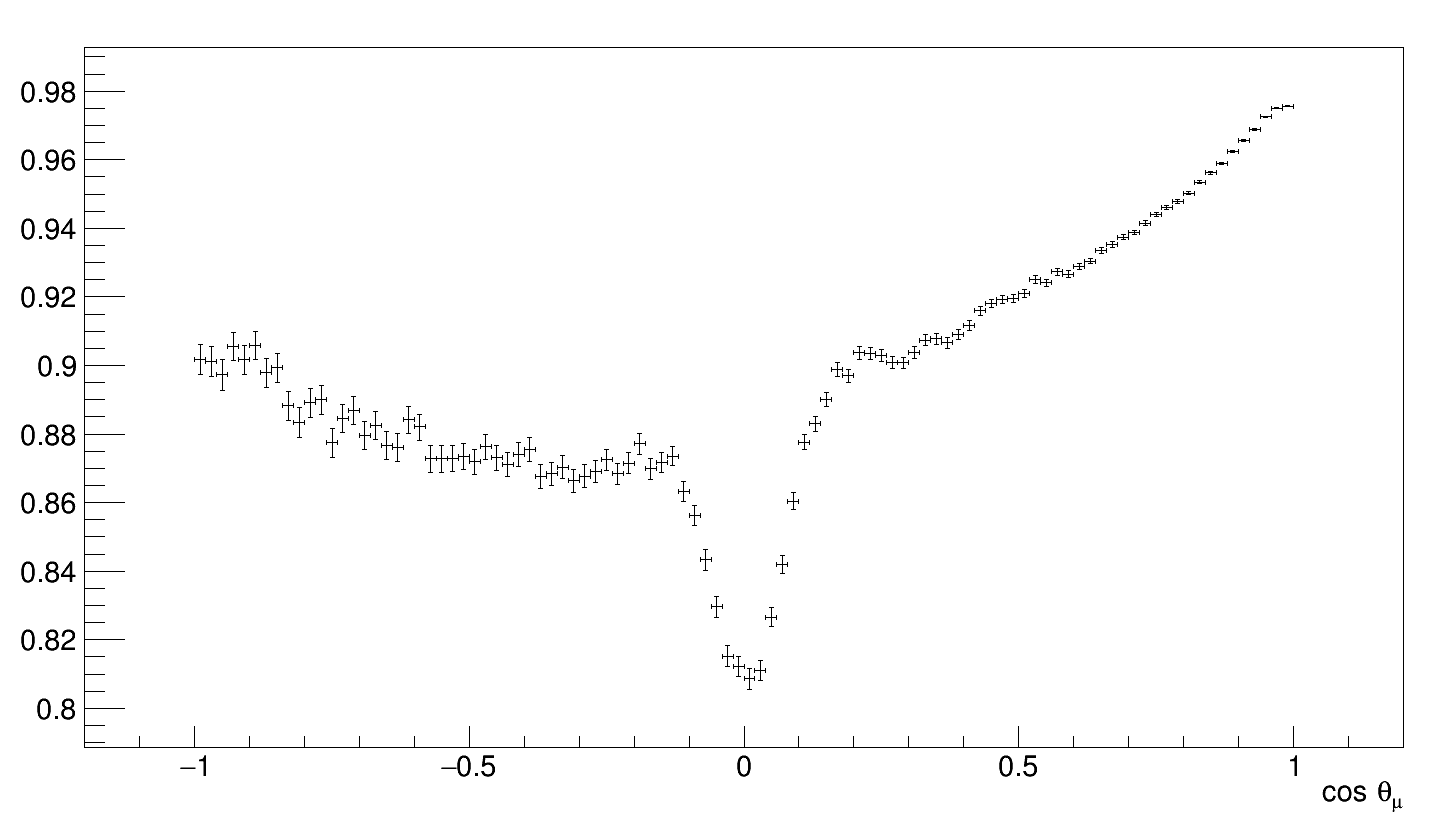
\includegraphics[width=0.45\textwidth]{plots.old/fig16.png}
    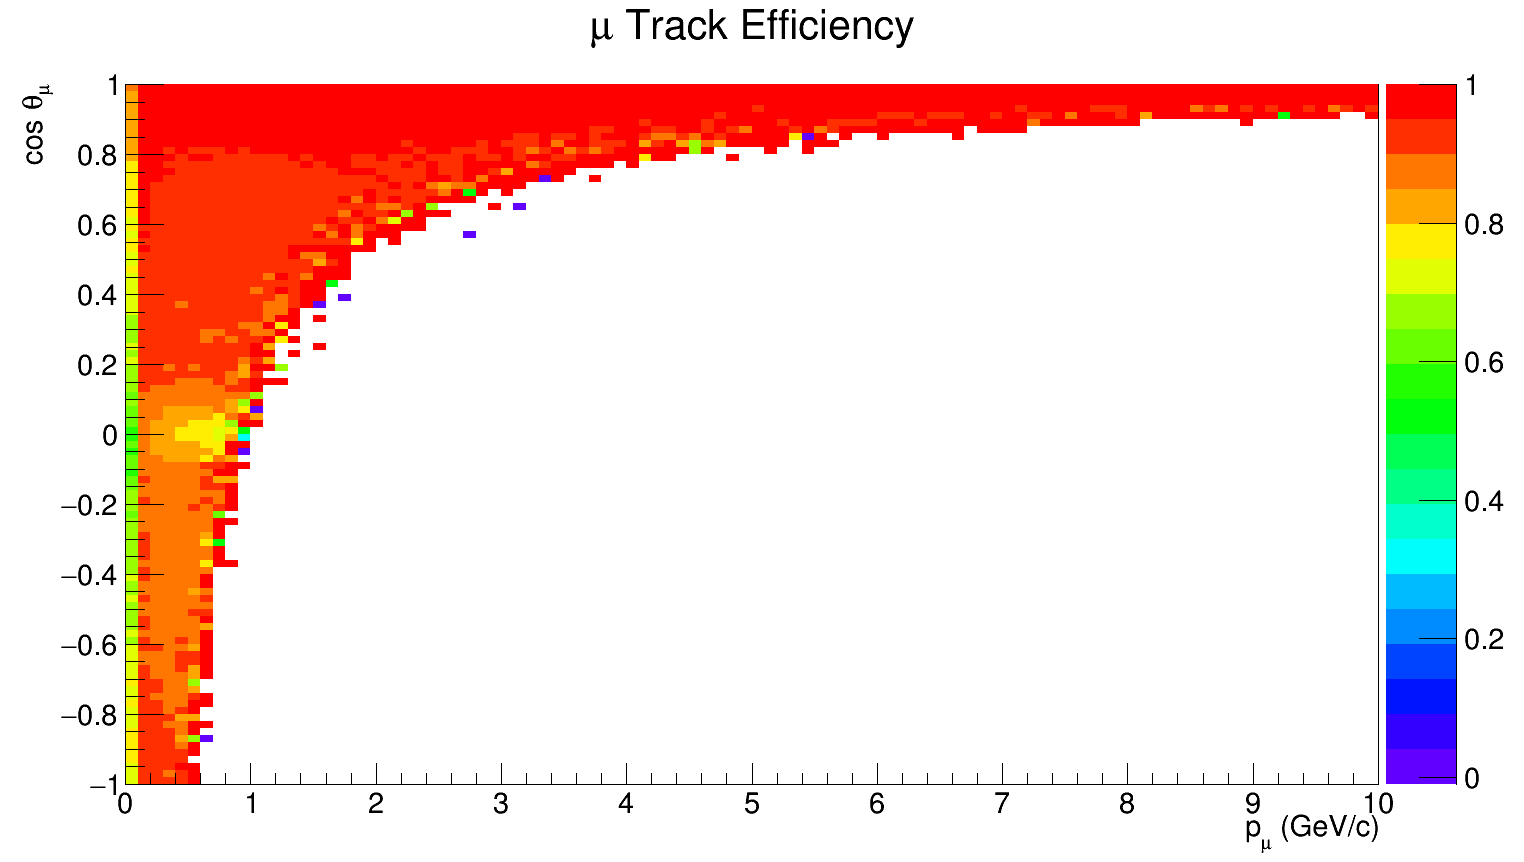
\includegraphics[width=0.5\textwidth]{plots.old/fig17.png}
    \caption{Reconstruction efficiency of muons as a function of $p_\mu$, $\cos \theta_\mu$ and both, calculated from NDTF files.}
  \end{center}
\end{figure}

These efficiencies can be applied to the same simulation as above to produce similar plots:

\begin{figure}[!h]
  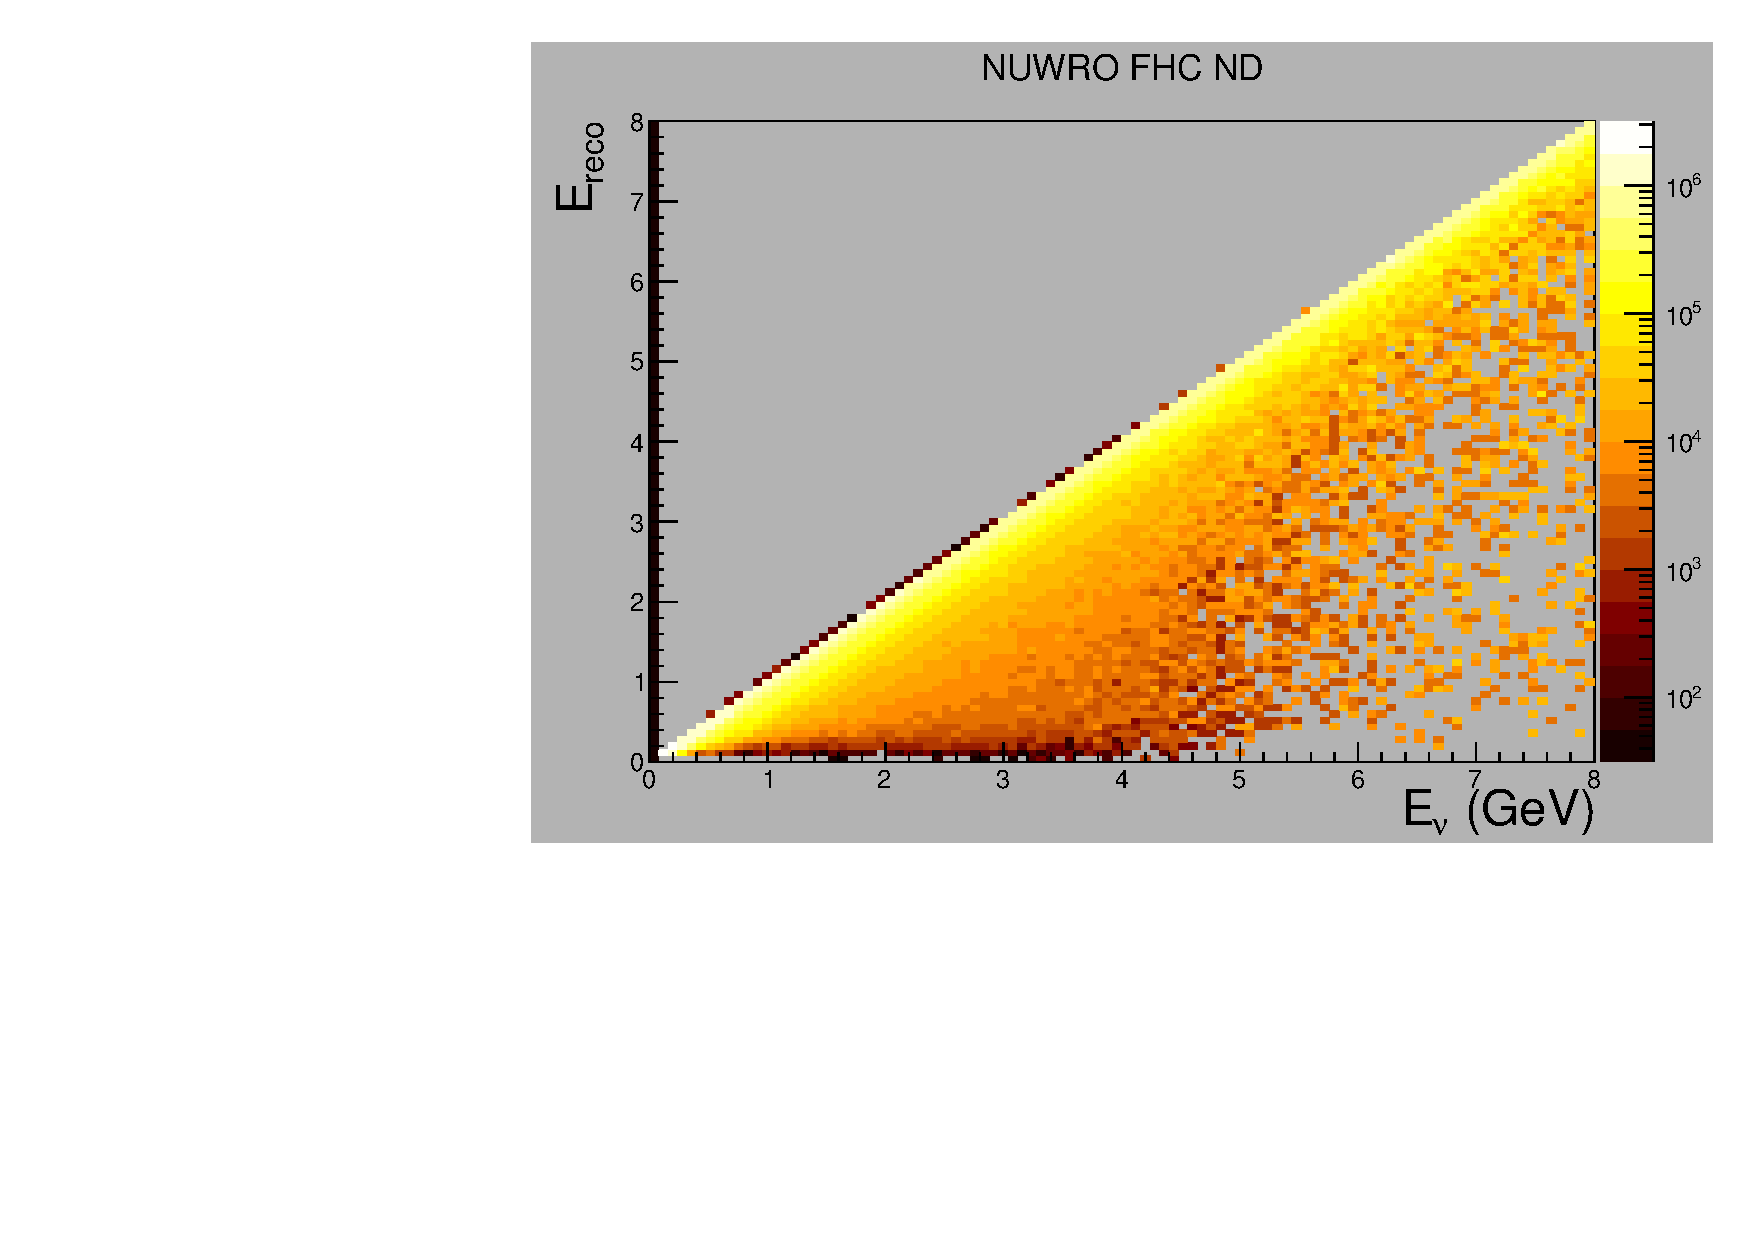
\includegraphics[width=0.5\textwidth]{plots.old/fig18.pdf}
  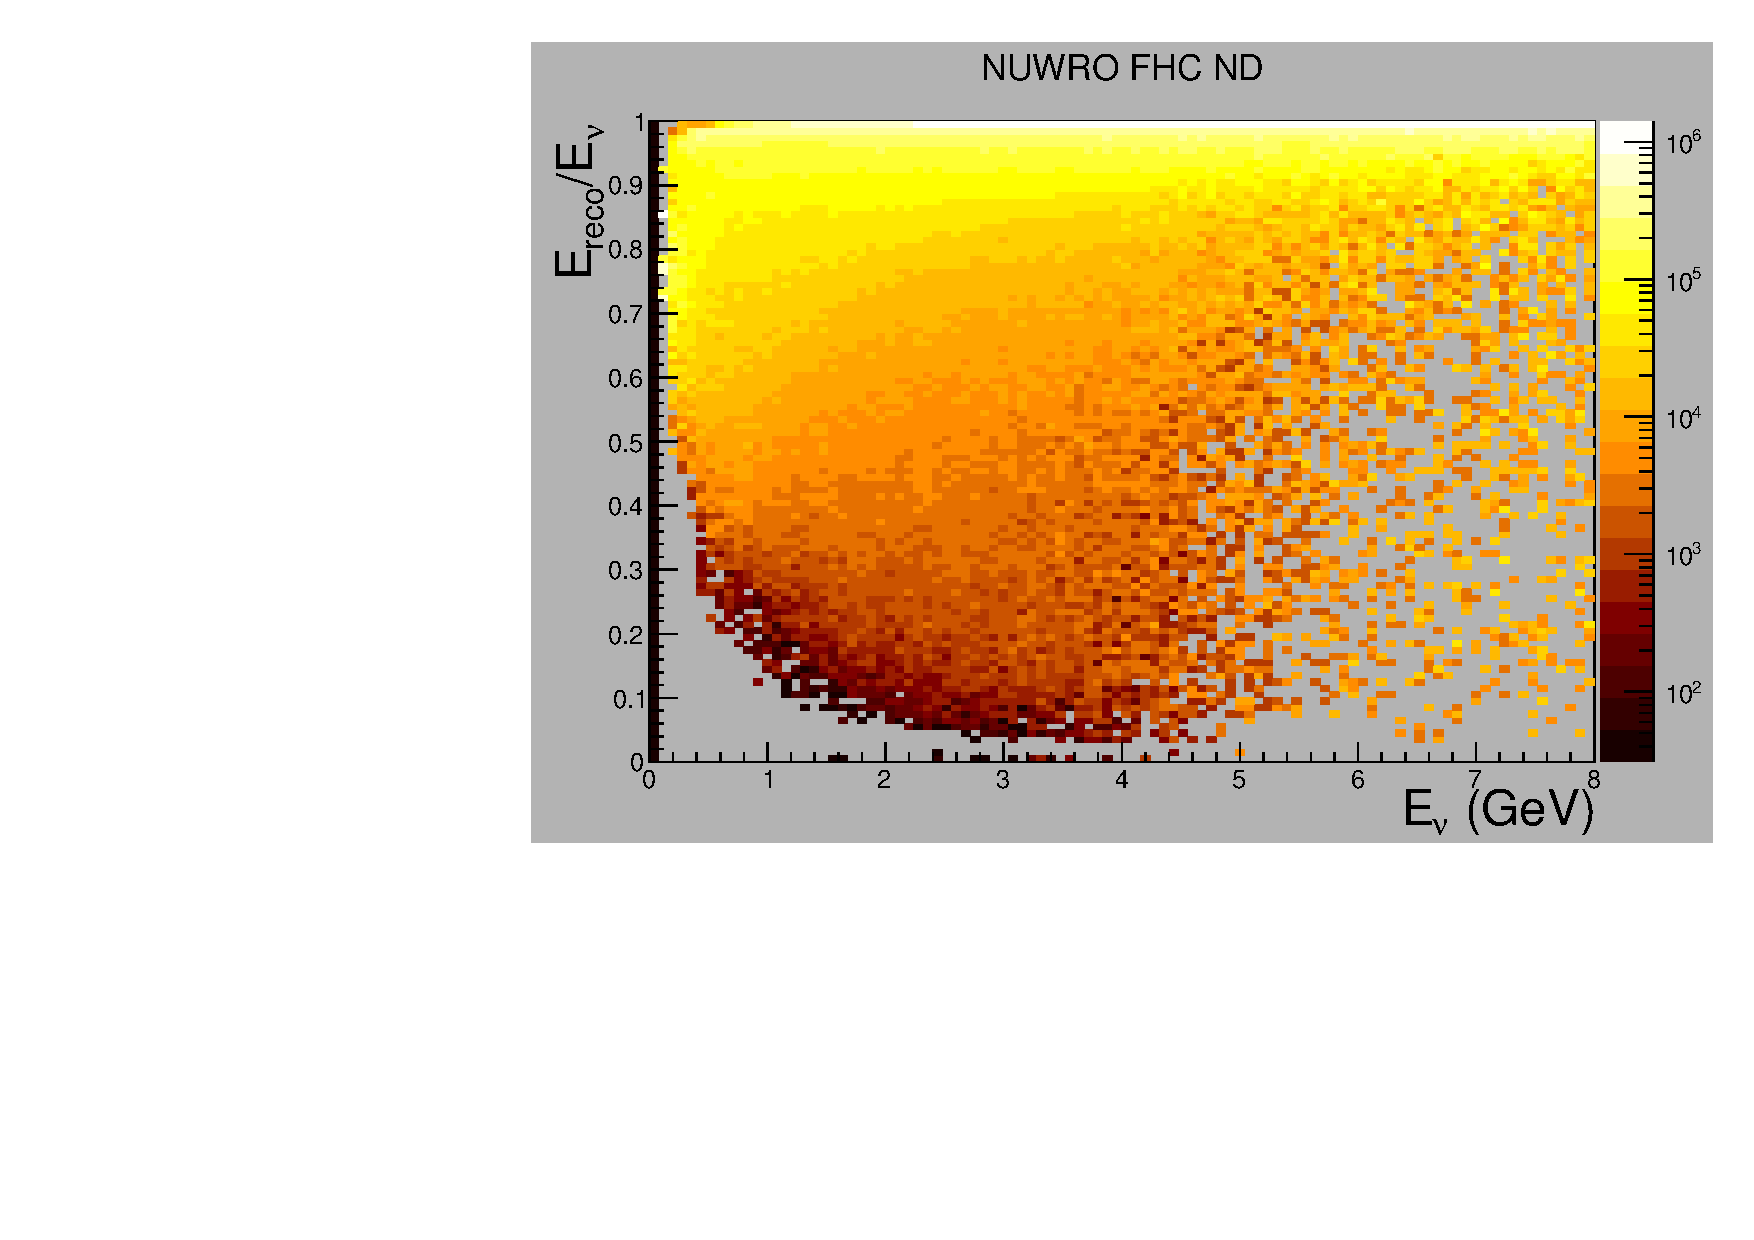
\includegraphics[width=0.5\textwidth]{plots.old/fig19.pdf}
  \caption{$E_{\mathrm{reco}}$ vs. $E_\nu$ shown for NUWRO events with FGT efficiency binned in $p$.}
\end{figure}

\begin{figure}[!h]
  \begin{center}
    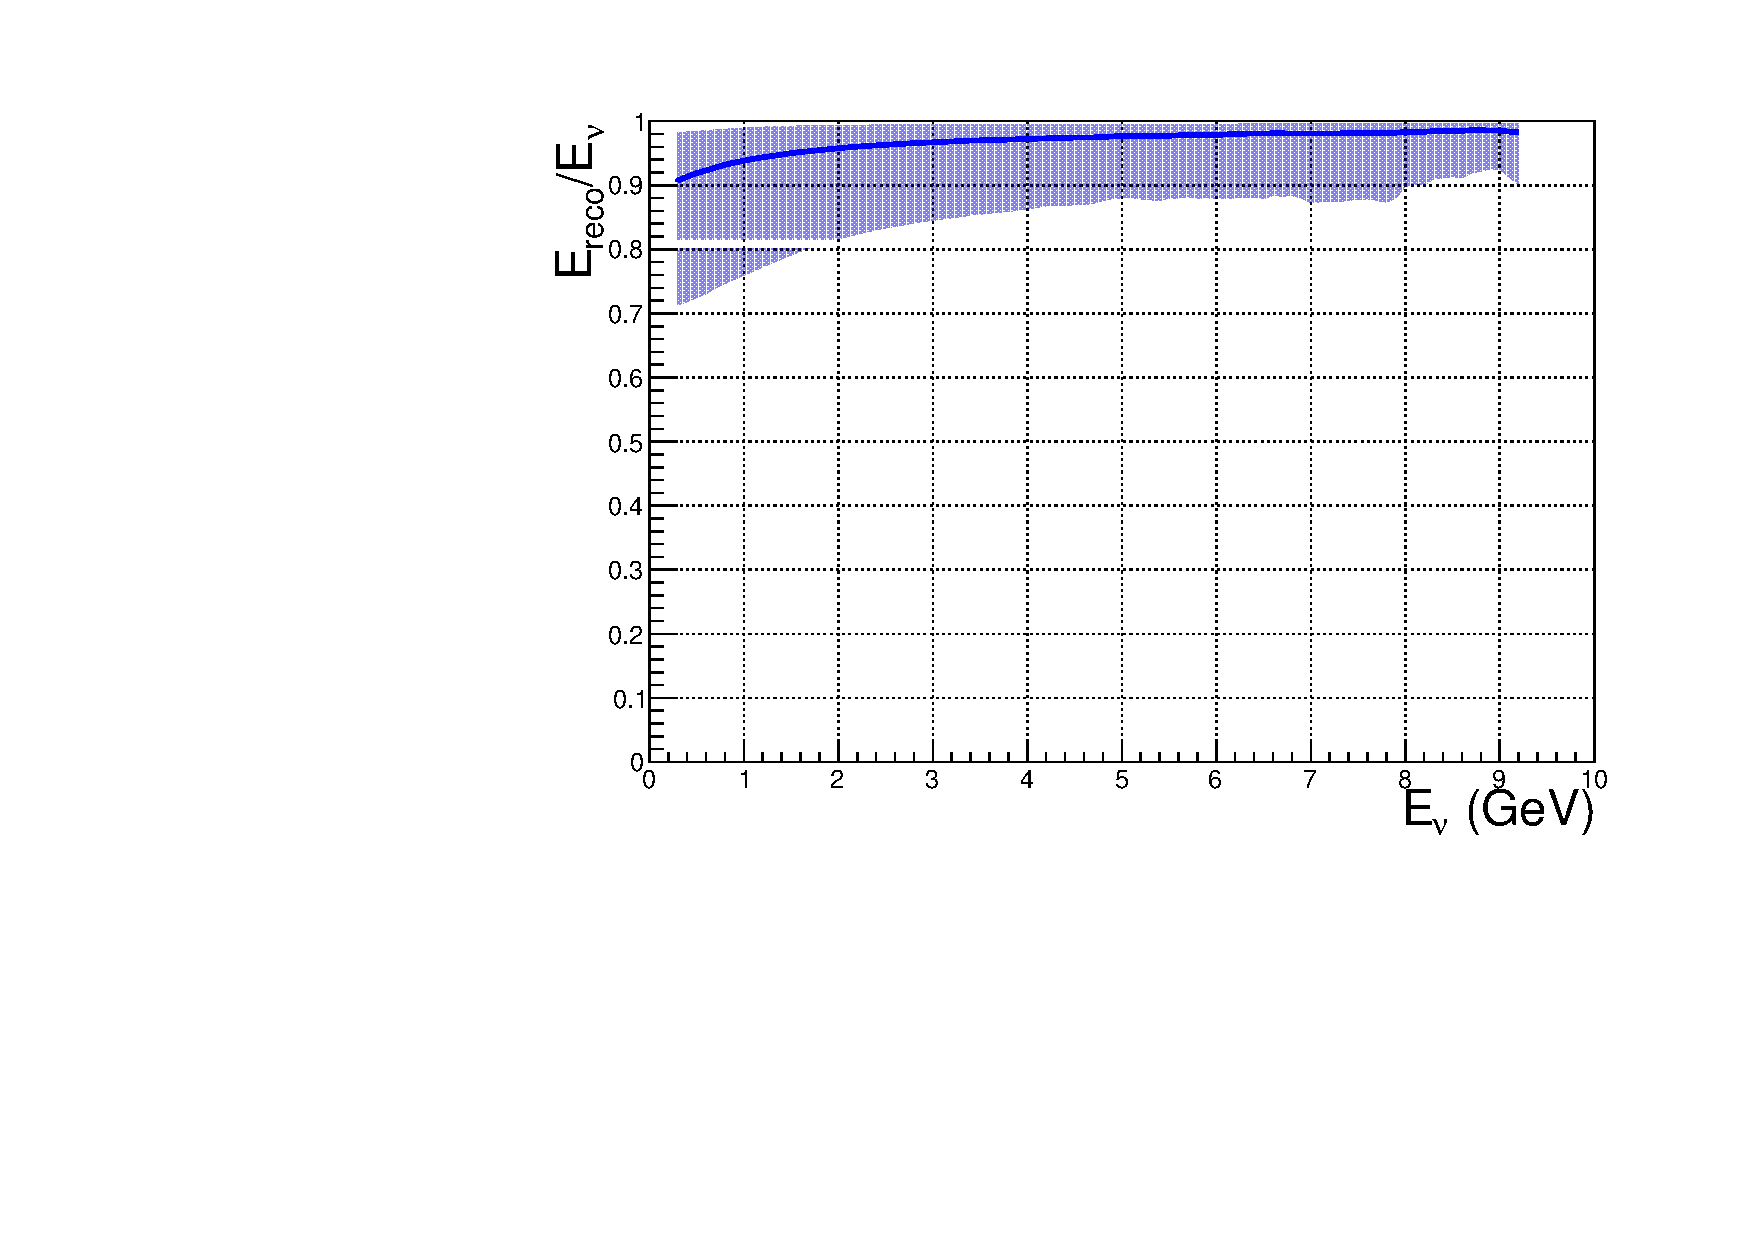
\includegraphics[width=0.7\textwidth]{plots.old/fig20.pdf}
    \caption{Median $E_{\mathrm{reco}}/E_\nu$ vs. $E_\nu$ for the above events with $68\%$ containment bands.}
  \end{center}
\end{figure}

\begin{figure}[!h]
  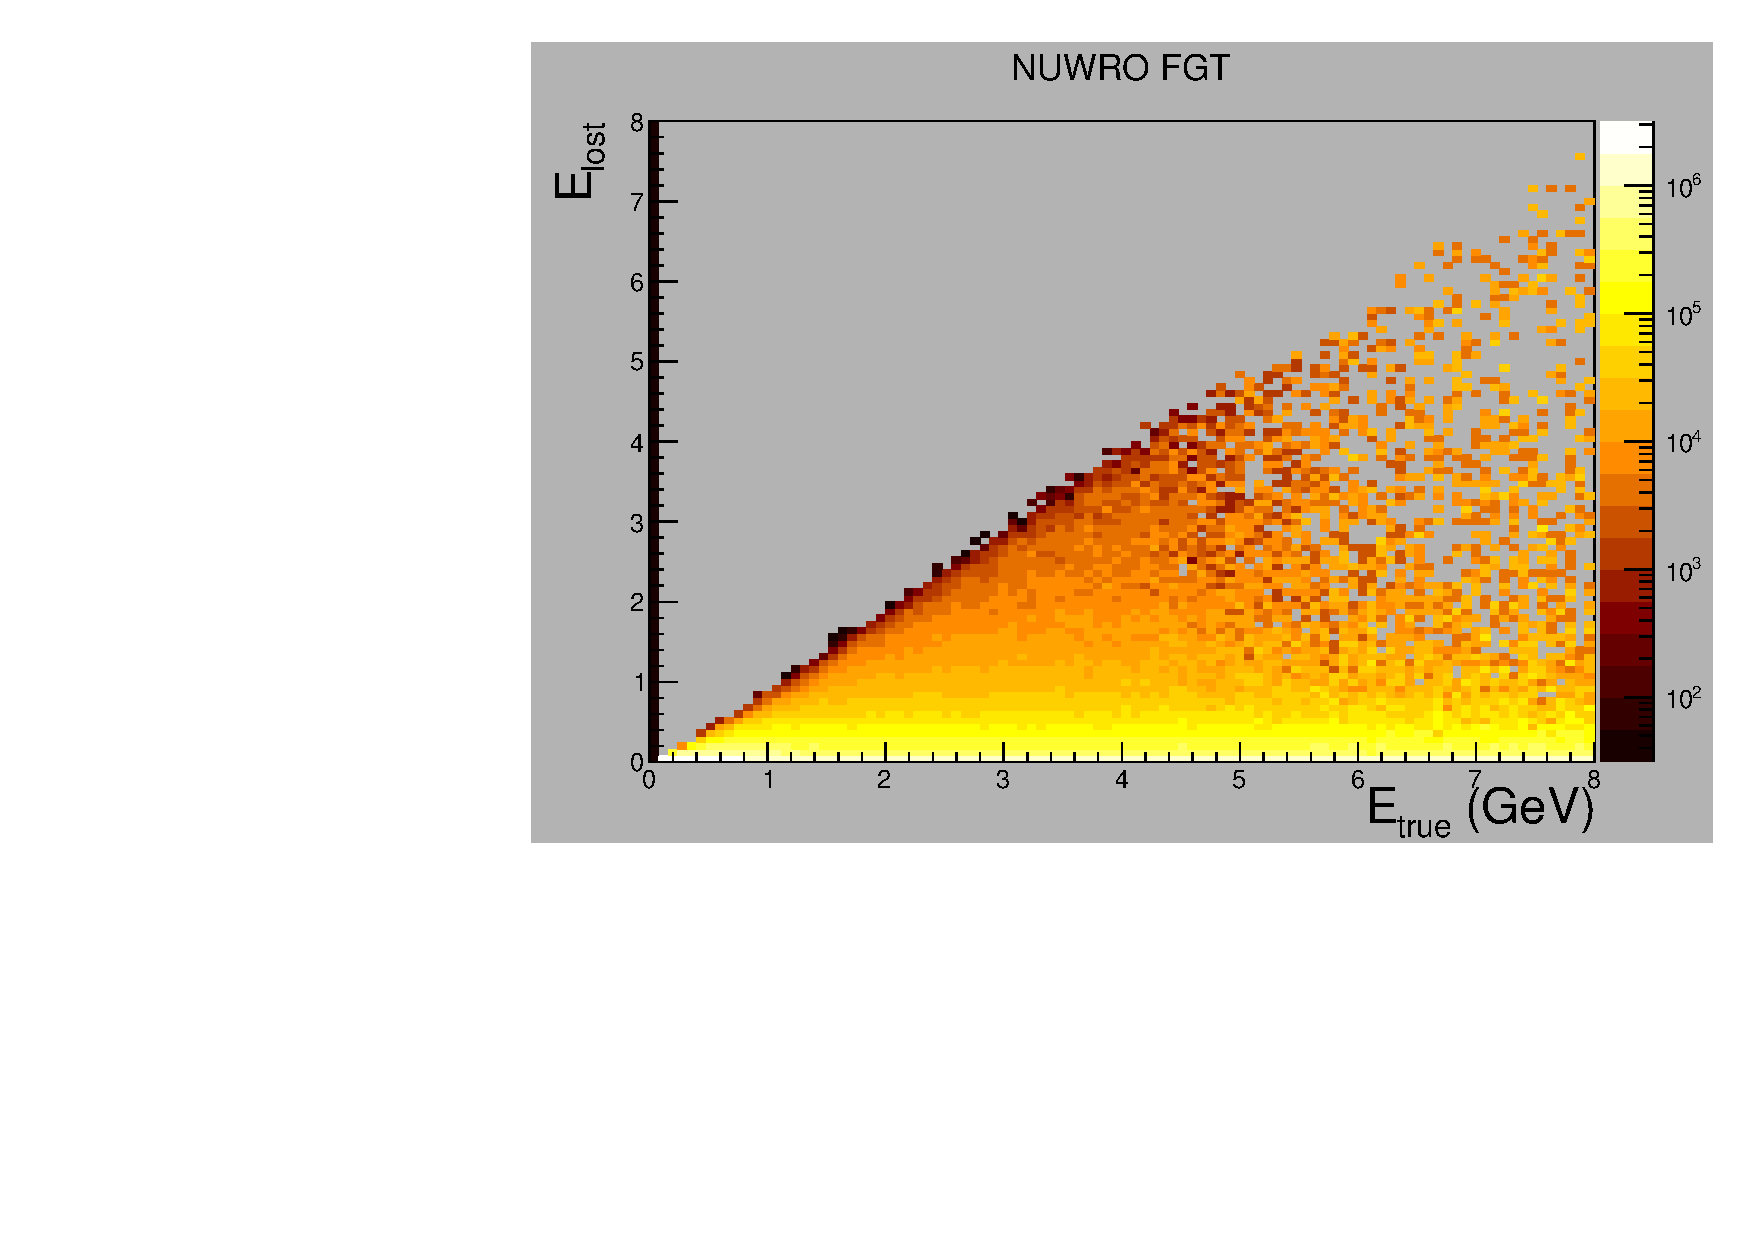
\includegraphics[width=0.5\textwidth]{plots.old/fig21.pdf}
  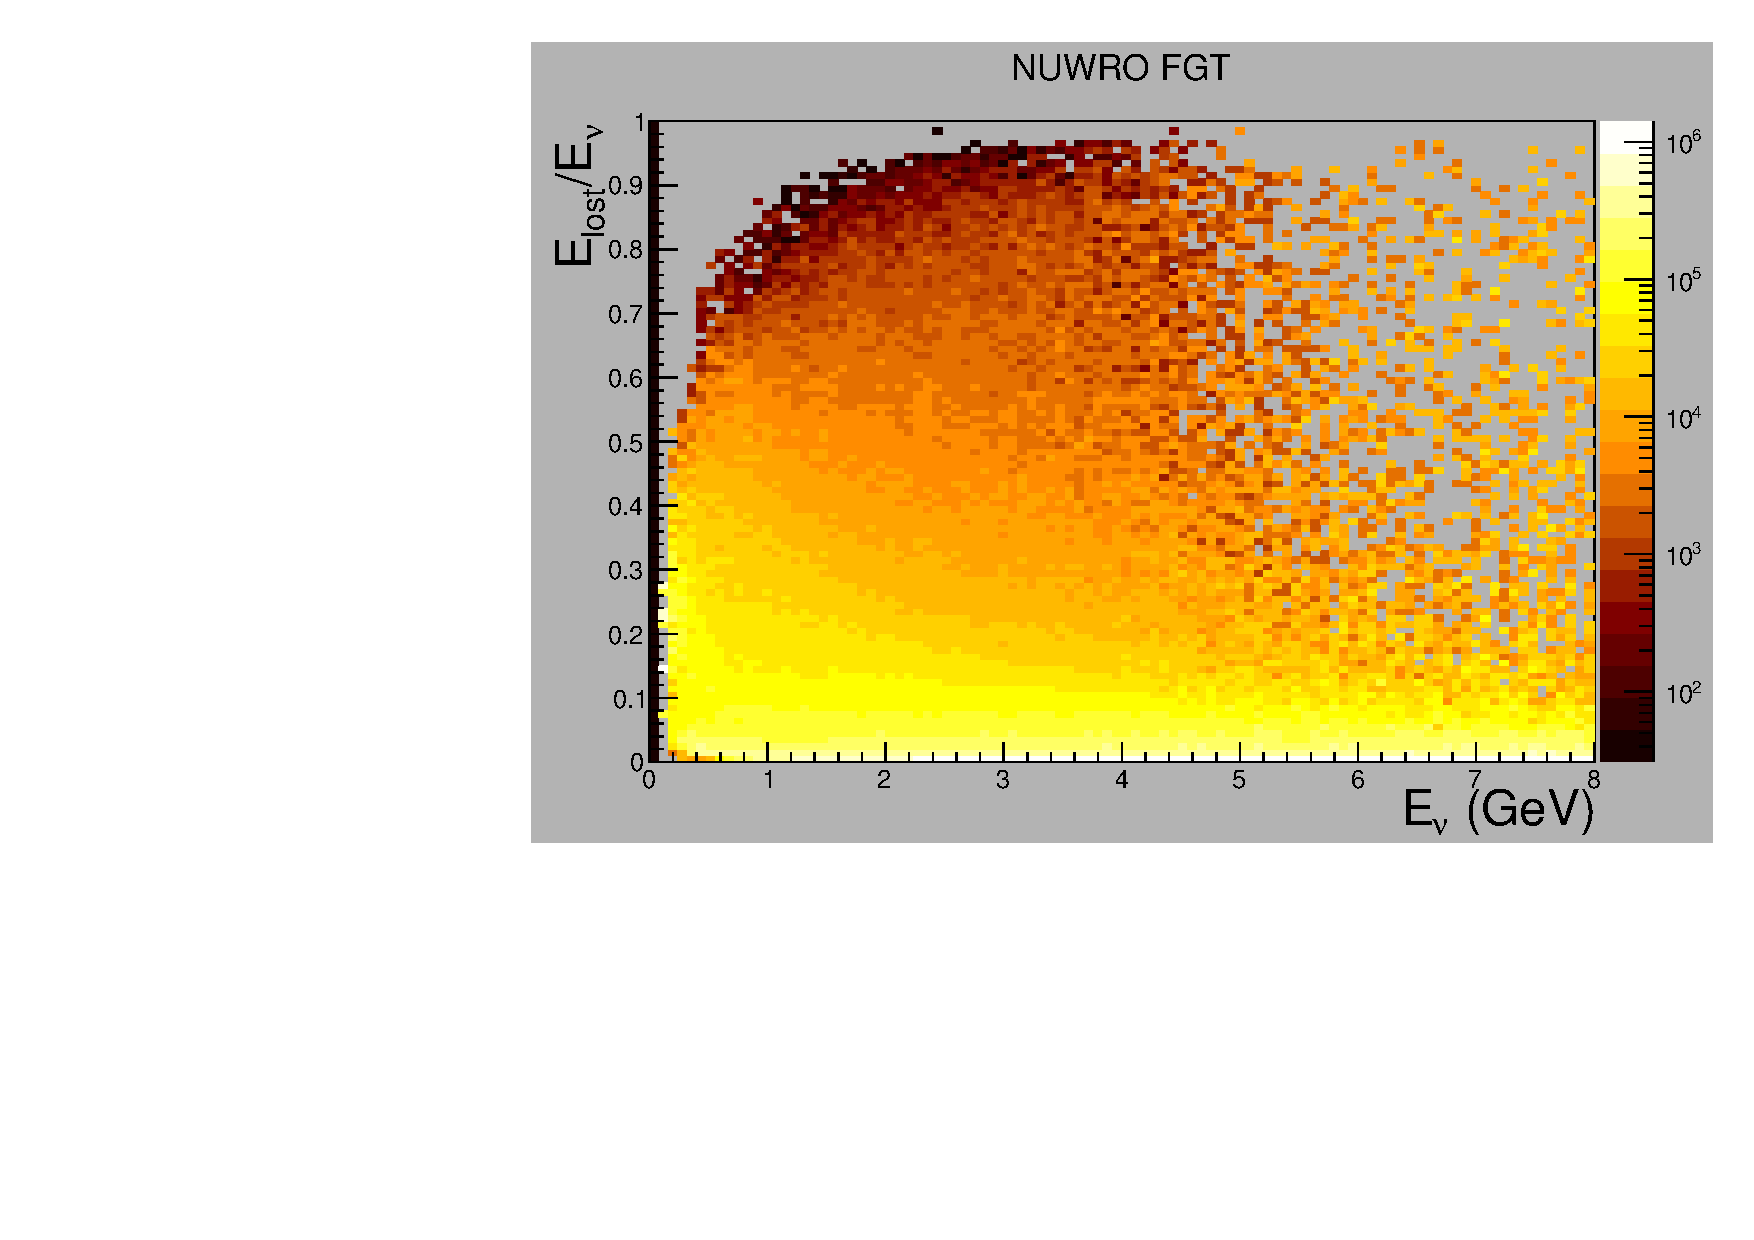
\includegraphics[width=0.5\textwidth]{plots.old/fig22.pdf}
  \caption{$E_{\mathrm{lost}}$ vs. $E_\nu$ shown for NuWro events with FGT efficiency binned in $p$.}
\end{figure}

\begin{figure}[!h]
  \begin{center}
    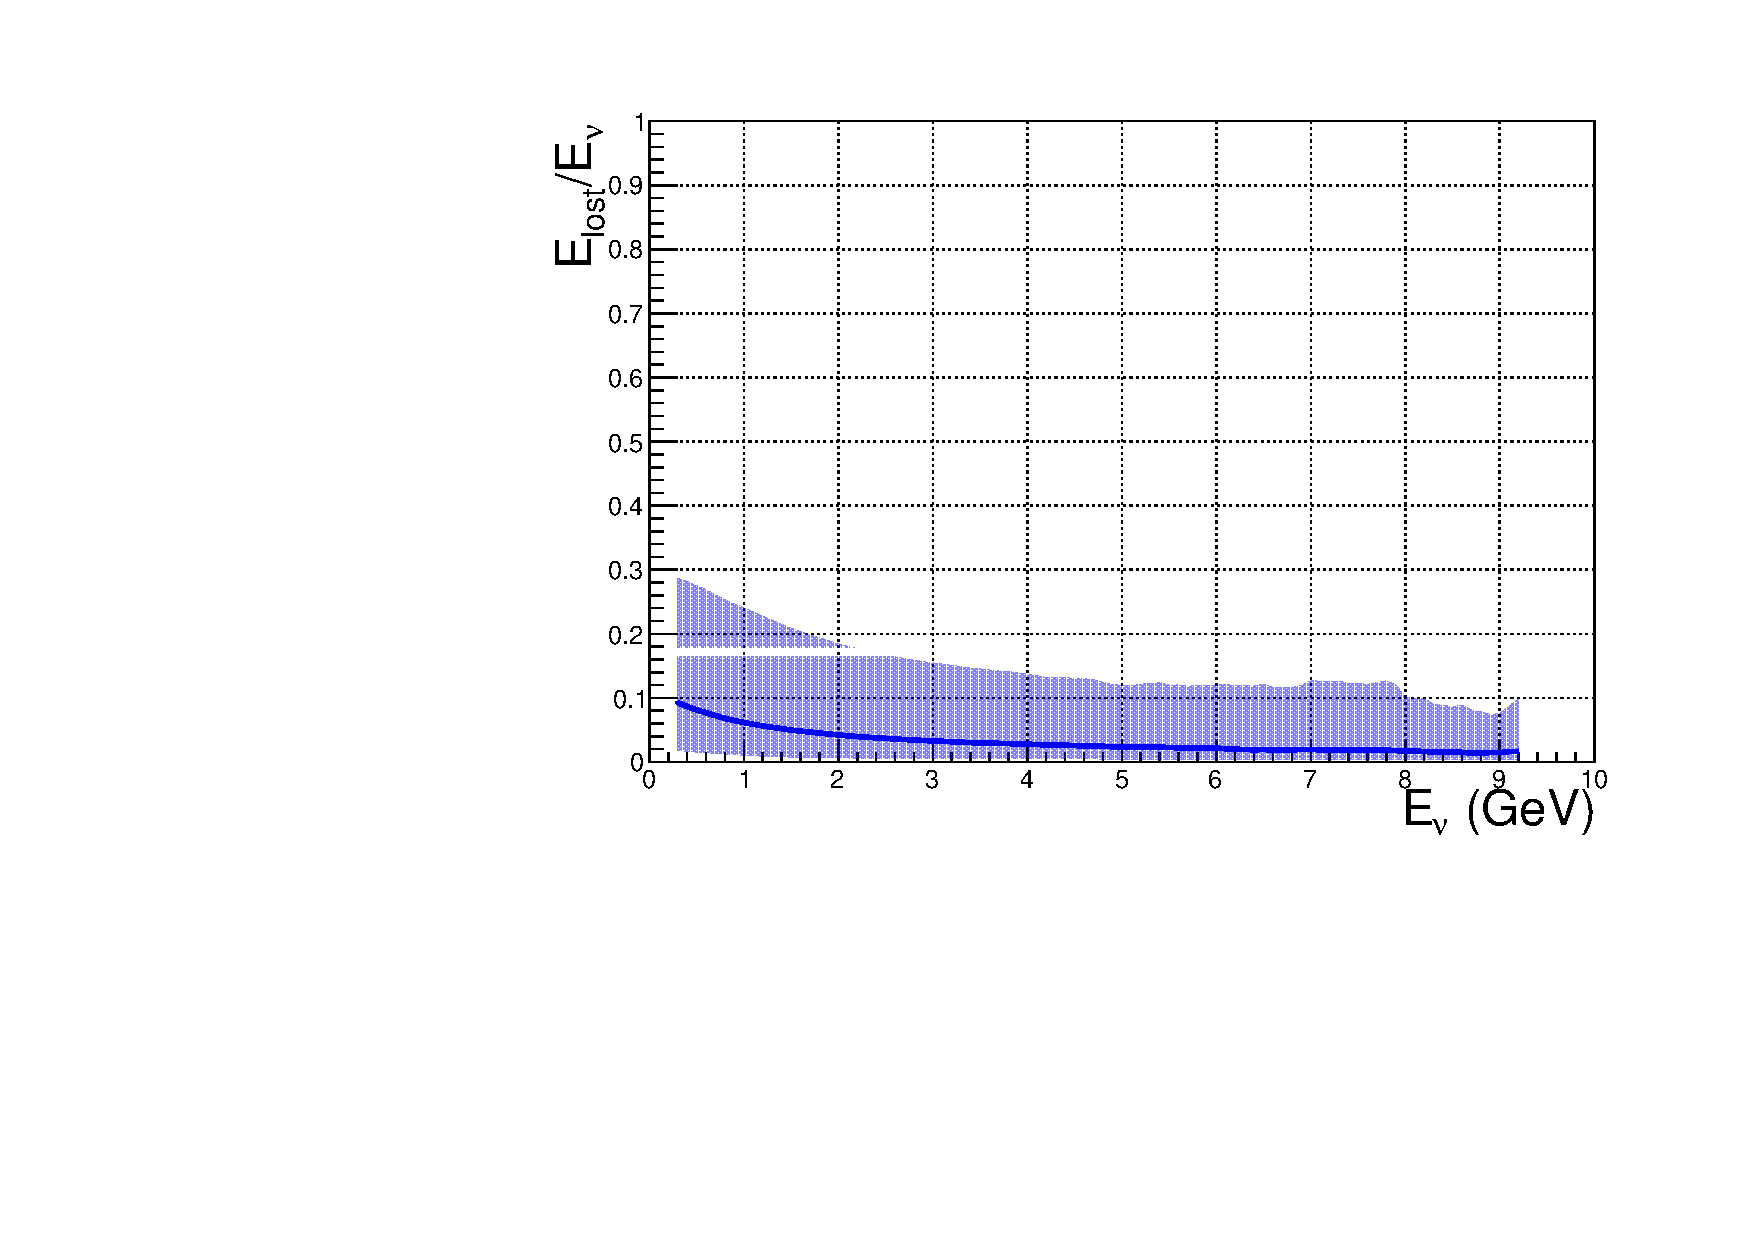
\includegraphics[width=0.7\textwidth]{plots.old/fig23.pdf}
    \caption{Median $E_{\mathrm{lost}}/E_\nu$ vs. $E_\nu$ for the above events with $68\%$ containment bands (NOTE: needs breakdown by FS particle).}
  \end{center}
\end{figure}

\subsubsection{LAr Efficiency}

\begin{figure}
  \begin{center}
    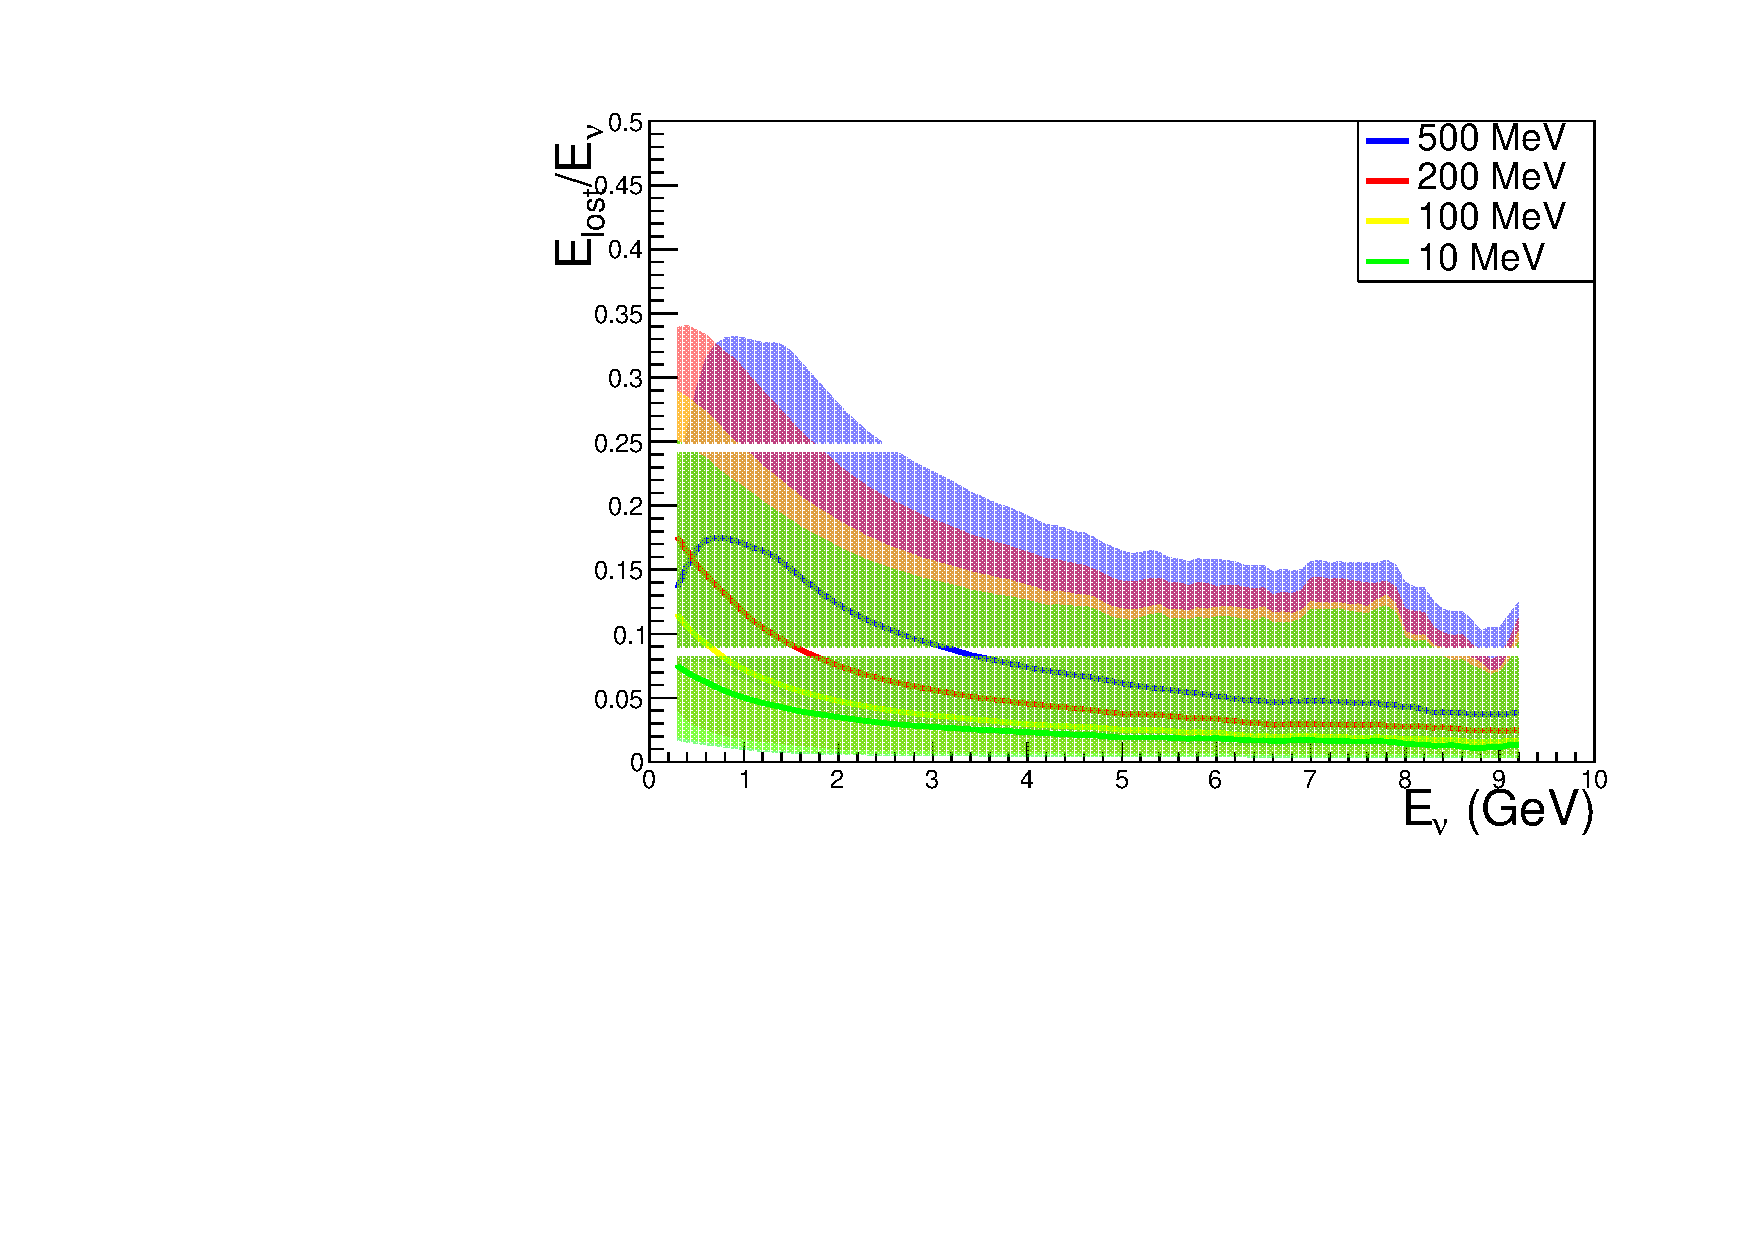
\includegraphics[width=0.7\textwidth]{plots.old/fig24.pdf}
    \caption{$E_{\mathrm{lost}}/E_\nu$ comparison using LAr efficiency gathered from microBooNE\textsuperscript{[citation needed]} TDR}
  \end{center}
\end{figure}

%% I have tons more plots that could be included here (other channels, RHC numub, each generator).  I'm not sure if I should include them all in an appendix.  As it is, I think this is very plot-dense and I'm not sure how to round it out.

\end{document}
